
In the final state, there are four jets, one charged lepton and \MET.
Various selections cuts are applied to ensure the resulting events to have 
this topology. Cutflow plots after various selection cuts are shown in 
Figure~\ref{fig:cutflow}. Below we list out various selection requirements applied.
\begin{enumerate}[leftmargin=*]
\item{\bf{Event filter and trigger}}:
    The events are passed to the filters and triggers (Section~\ref{ss:secTrig}). 
    The lepton trigger is used to enrich events with lepton and significantly reduces QCD multijet 
    compared to other SM background. The number of events surviving filters and trigger cuts for 
    simulated signal and background and data are shown in the 2nd column of Tables
\ref{tab:cutflow_mu}, \ref{tab:cutflow_ele}, \ref{tab:cutflow_mu_sig} and \ref{tab:cutflow_ele_sig}. 
\item {\bf{Lepton selection}}:
The event topology has only one lepton thus events having a second loose lepton are not selected. 
The lepton-veto selection for the \mujets and \ejets channel are listed in Tables~\ref{tab:muonSel}
and \ref{tab:eleSel}.
For the \mujets (\ejets) channel there cannot be any electron (muon) in an event.
Those events where there is any electron (muon) in the \mujets (\ejets) channel are rejected.
Lepton scale factors as described in Section~\ref{s:lepton_sf} are applied to the simulated events.
The relative isolation cut for muon is $I_{\rm {rel}}^{\mu} < 0.15$ and for electron it is 
$I_{\rm {rel}}^{\rm{e}} < 0.0821 (0.0695)$ in the barrel (endcap) region.
Event yields after one lepton selection are shown in the 3rd column of Tables~\ref{tab:cutflow_mu},
\ref{tab:cutflow_ele}, \ref{tab:cutflow_mu_sig} and \ref{tab:cutflow_ele_sig}.

\item {\bf{Jet selection}}:
There should be at least four jets in an event.
Jet selection cuts are listed in Table~\ref{tab:jetSel}.
The jet energy is corrected using JES and JER scale factors.
After correcting jet energy, the selections on jet as shown in Table~\ref{tab:jetSel} are applied.
Number of events after jet selection are shown in the 4th column of Tables~\ref{tab:cutflow_mu},
\ref{tab:cutflow_ele}, \ref{tab:cutflow_mu_sig} and \ref{tab:cutflow_ele_sig}.

\item {\bf{\MET selection}}:
The missing transverse energy should be greater than 20 \GeV. Event yields after \MET selection are 
shown in the 5th column of Tables~\ref{tab:cutflow_mu}, \ref{tab:cutflow_ele}, \ref{tab:cutflow_mu_sig}
and \ref{tab:cutflow_ele_sig}. After applying \MET selection QCD multijet, \dyjets event yields reduce 
more compared to \ttjets, single \PQt, \wjets, and VV processes as there is no neutrino at the parton level.

\item {\bf{\text{b} jet selection}}:
For \PQb jet selection, the medium working point is used i.e, $b_{\text{discr}} > 0.8484$. 
The \PQb tag event weights, as described in Section~\ref{s:bTagSF}, are applied on simulated events. 
The events are required to have at least two \PQb jets. Event yields for simulated signal, background 
and data are shown in the 6th column of Tables~\ref{tab:cutflow_mu}, \ref{tab:cutflow_ele}, 
\ref{tab:cutflow_mu_sig} and \ref{tab:cutflow_ele_sig}.
\end{enumerate}

From Table~\ref{tab:cutflow_mu} (\ref{tab:cutflow_ele}) it can be seen that the \wjets 
process is the dominant background upto 1-lepton selection. However, when the events are 
required to have $N_{\rm{jets}} \geq 4$, the \ttjets becomes the dominant background. The \ttjets 
remains dominant background after subsequent selection cuts. The QCD multijet events are from
simulated samples as shown in Table~\ref{tab:mcSample}. The signal event yields for a different 
mass of charged Higgs after various selection cuts are shown in Table~\ref{tab:cutflow_mu_sig}
(\ref{tab:cutflow_ele_sig}) for the \mujets (\ejets) channel. It can be seen from these tables 
that the event yields are almost the same upto 1-lepton selections for all masses of charged Higgs. 
However, after the $N_{\text{jets}} \geq 4$ selection, when \ttjets becomes the dominant 
background as shown in Table~\ref{tab:cutflow_mu} (\ref{tab:cutflow_ele}), the event yield 
for higher masses of the charged Higgs are reduced more compared to lower masses. The 
event yield reduces because of the less phase space available between \PQt quark and charged 
Higgs for higher masses.
    
\begin{center}
\begin{figure}
\subfigure[]{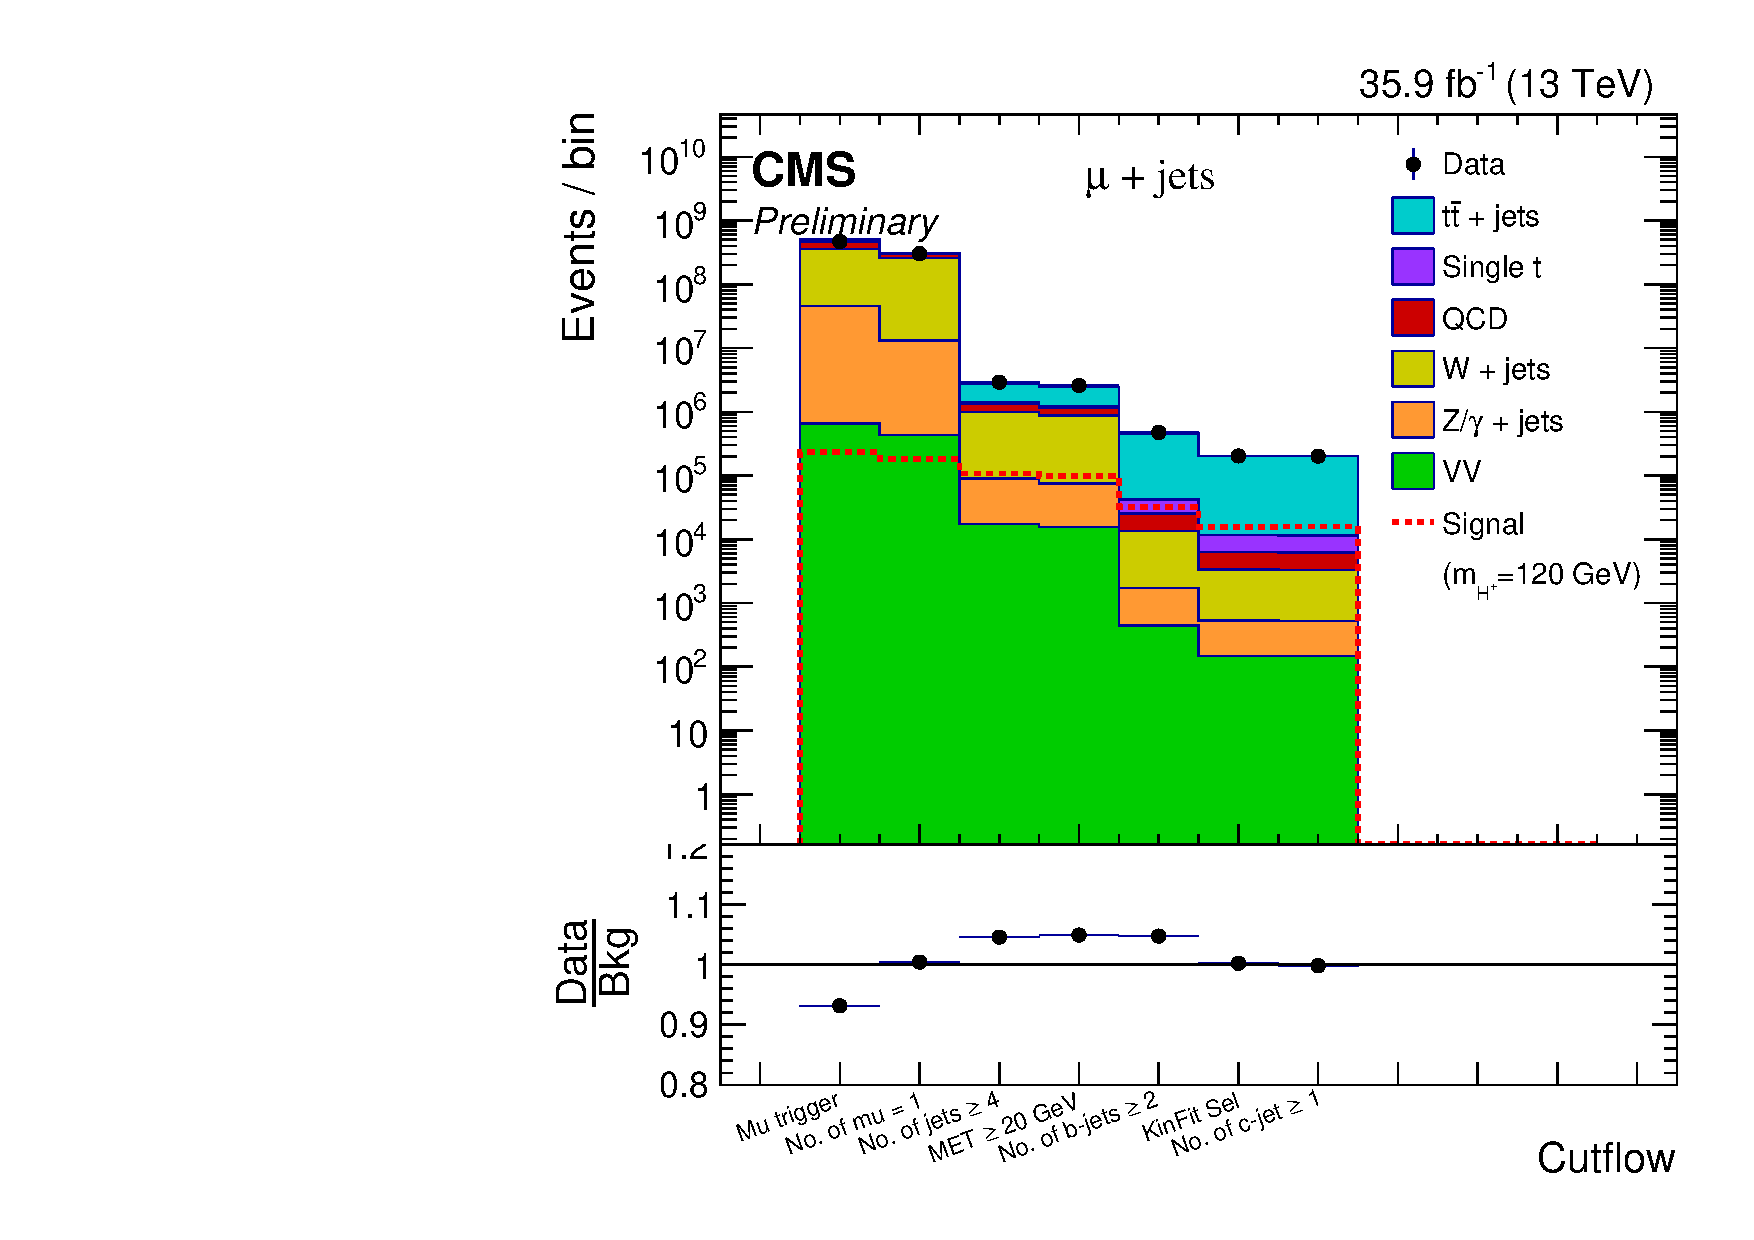
\includegraphics[width=0.50\linewidth]{Image/Muon/cutflow_mu.pdf}}
\subfigure[]{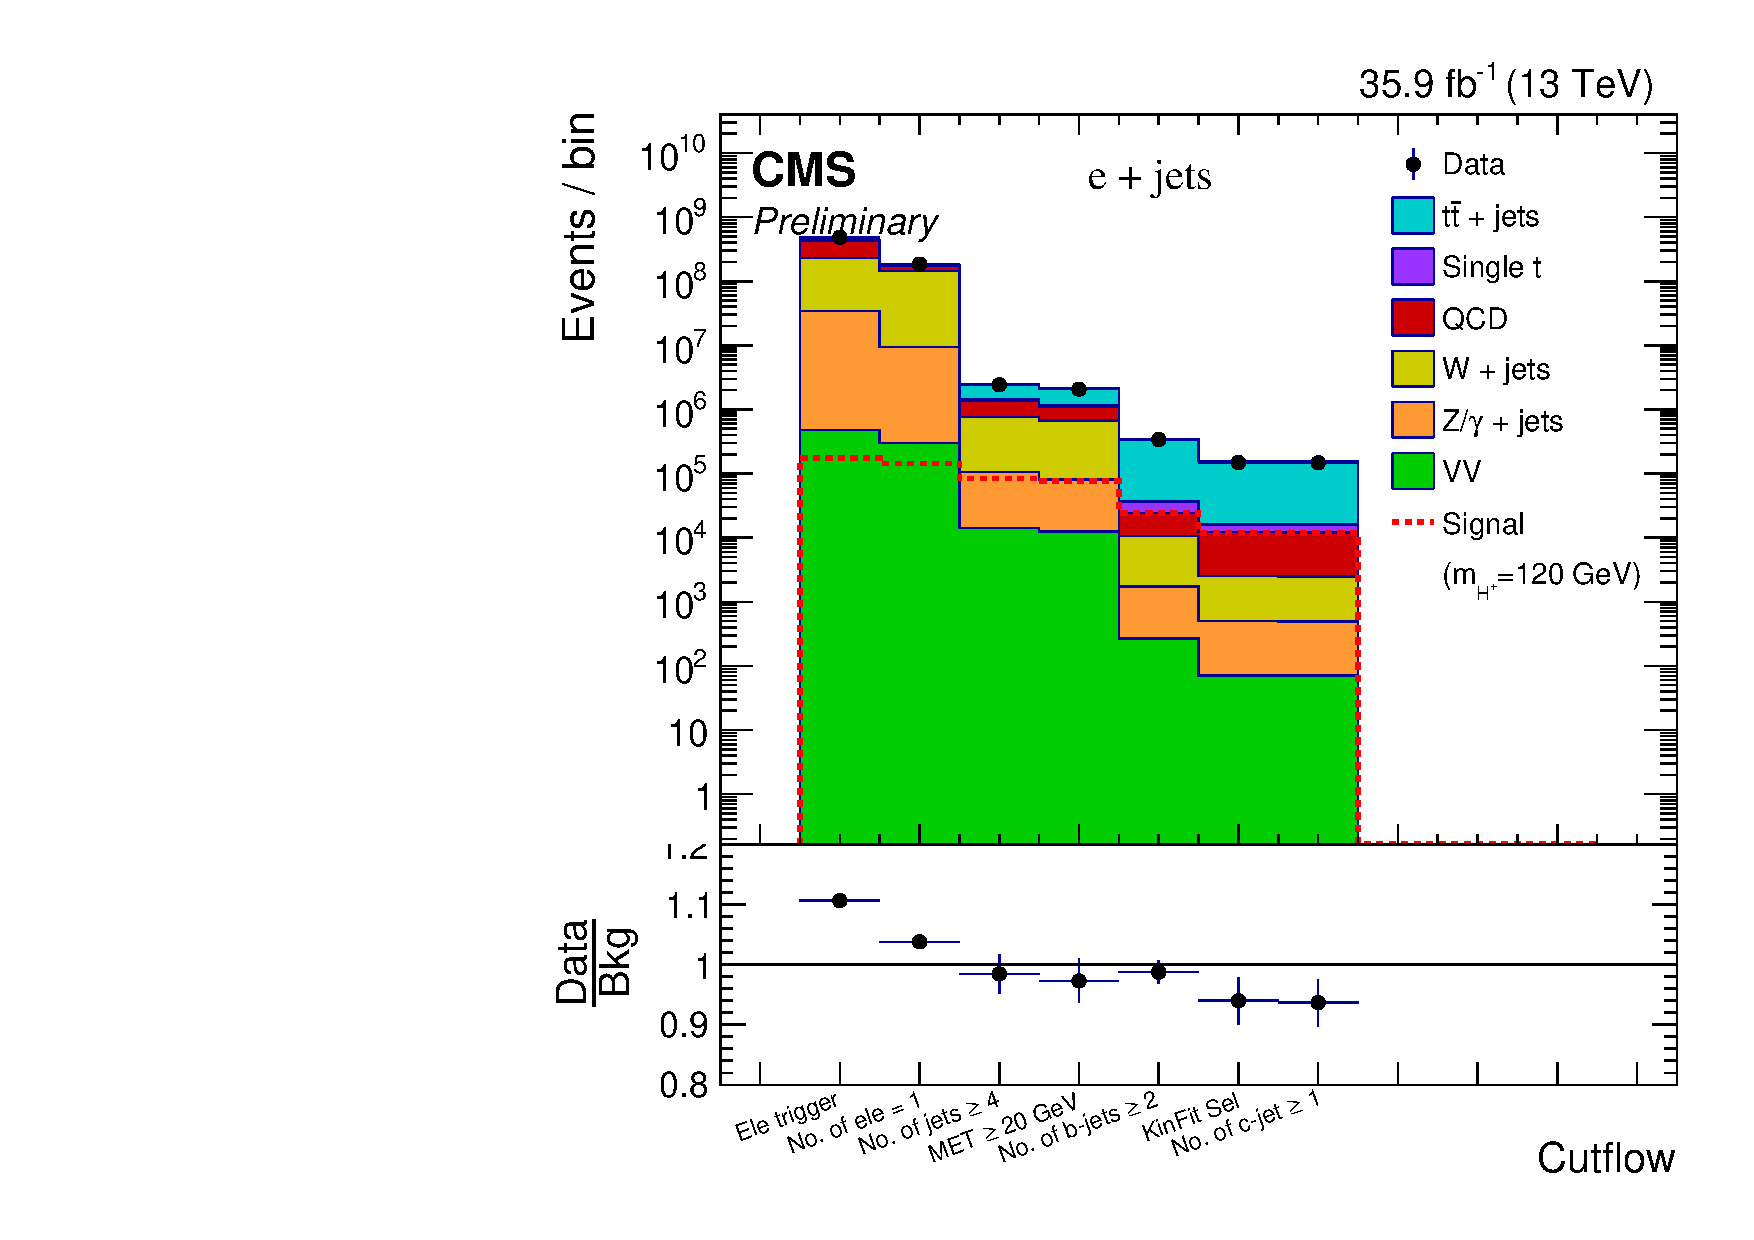
\includegraphics[width=0.50\linewidth]{Image/Electron/cutflow_ele.pdf}}
\caption{ Event yields after various selection cuts for the \mujets and \ejets channel.} 
\label{fig:cutflow}
\end{figure}
\end{center}

\begin{table}
\begin{center}
    \caption{Event yields after various selection cuts for the \mujets
    channel. The \wjets process is the dominant background upto 1-lepton 
    selection. When the events are required to have $N_{jets} \geq 4$, the 
    \ttjets becomes the dominant background. The QCD multijet events are 
    from simulated samples as listed in Table~\ref{tab:mcSample}. The simulated 
    MC signal process corresponds to $\mHp=120$ \GeV.}
\label{tab:cutflow_mu}
\begin{adjustbox}{max width=\textwidth}
\begin{tabular}{cccccccc}
\hline 
\hline 
\multicolumn{1}{ c}{Process } & \multicolumn{1}{ c}{ Trigger } & \multicolumn{1}{ c}{ $N_{\mu}=1$ } &\multicolumn{1}{ c}{ $N_{\rm{jets}}\ge 4$ } & \multicolumn{1}{ c}{ $\MET \ge $ 20\GeV }&  \multicolumn{1}{ c }{ $\ge$ 2 \PQb jets }& \multicolumn{1}{ c}{KF selection } & \multicolumn{1}{ c}{ $\ge$1 \PQc jet} \\ 
\hline 
\hline 
MC signal & 232088 & 182966 & 107237 & 97792 & 32309 & 15719.1 & 15784.7 \\ 
\hline 
SM \ttjets & 4.02837e+06 & 2.6683e+06 & 1.36181e+06 & 1.24994e+06 & 411521 & 191136 & 190228 \\ 
Single t\PQt & 589196 & 428074 & 81804 & 74924.6 & 16599.5 & 5311.76 & 5272.39 \\ 
\wjets & 3.09765e+08 & 2.44546e+08 & 894318 & 797849 & 11767.7 & 2795.35 & 2760.97 \\ 
\dyjets & 4.48481e+07 & 1.27487e+07 & 73347.7 & 59133.7 & 1272.68 & 389.494 & 377.772 \\ 
QCD multijet & 1.4453e+08 & 4.07546e+07 & 355254 & 265303 & 11962.6 & 3007.9 & 2960.23 \\ 
VV & 653661 & 433207 & 17232.4 & 15614.6 & 440.143 & 146.569 & 146.862 \\ 
\hline 
Bkg & 5.04414e+08 & 3.01579e+08 & 2.78377e+06 & 2.46276e+06 & 453564 & 202787 & 201746 \\ 
\hline 
Data & 4.69828e+08 & 3.02791e+08 & 2.91052e+06 & 2.58346e+06 & 475011 & 203209 & 201361 \\ 
\hline 
Data/Bkg & 0.931433 & 1.00402 & 1.04553 & 1.04901 & 1.04729 & 1.00208 & 0.998092 \\ 
\hline 
\end{tabular}
\end{adjustbox}
\end{center}
\end{table}

\begin{table}
\begin{center}
    \caption{Event yields after various selection cuts for the \ejets channel. A similar trend as 
that of Table~\ref{tab:cutflow_mu} is seen. The simulated MC signal process corresponds to $\mHp=120$ \GeV.}
\label{tab:cutflow_ele}
\begin{adjustbox}{max width=\textwidth}
\begin{tabular}{cccccccc}
\hline 
\hline 
\multicolumn{1}{ c}{Process } & \multicolumn{1}{ c}{ Trigger } & \multicolumn{1}{ c}{ $N_{\rm {e}}=1$ } &\multicolumn{1}{ c}{ $N_{\rm{jets}}\ge 4$ } & \multicolumn{1}{ c}{ $\MET \ge 20 \GeV$ }&  \multicolumn{1}{ c }{ $\ge$ 2 \PQb jets }& \multicolumn{1}{ c}{KF selection} & \multicolumn{1}{ c}{$\ge$1 \PQc jet} \\ 
\hline 
\hline 
MC signal & 176709 & 143701 & 83955.8 & 76103.8 & 24488.2 & 11805.2 & 11835.4 \\ 
\hline 
SM \ttjets & 3.00511e+06 & 2.04055e+06 & 1.03705e+06 & 949027 & 306375 & 141807 & 141111 \\ 
Single \PQt & 436844 & 314868 & 63532.5 & 57857.3 & 12741.7 & 3988.54 & 3953.51 \\ 
\wjets & 1.95739e+08 & 1.34112e+08 & 660657 & 586662 & 8878.8 & 2031.55 & 1991.47 \\ 
\dyjets & 3.38256e+07 & 9.13592e+06 & 91830.9 & 68347.4 & 1449.81 & 433.03 & 418.256 \\ 
QCD multijet & 2.05104e+08 & 3.2298e+07 & 595856 & 453793 & 13497.6 & 9678.07 & 9613.93 \\ 
VV & 479881 & 298702 & 14058.6 & 12404.1 & 270.078 & 70.432 & 70.2293 \\ 
\hline 
Bkg & 4.3859e+08 & 1.782e+08 & 2.46299e+06 & 2.12809e+06 & 343213 & 158009 & 157158 \\ 
\hline 
Data & 4.85205e+08 & 1.84925e+08 & 2.42496e+06 & 2.07011e+06 & 338837 & 148500 & 147210 \\ 
\hline 
Data/Bkg & 1.10628 & 1.03774 & 0.984561 & 0.972755 & 0.98725 & 0.939821 & 0.936699 \\ 
\hline 
\end{tabular}
\end{adjustbox}
\end{center}
\end{table}

\begin{table} 
\begin{center} 
    \caption{Signal event yields for the different mass of charged Higgs after 
    various selection cuts for the \mujets channel. Event yields are almost
    same upto 1-lepton selection for all mass points. However, after the 
    $N_{jets} \geq 4$ selection (when \ttjets becomes the dominant
    background as shown in Table~\ref{tab:cutflow_mu}) the event yield for higher
    masses of the charged Higgs are reduced more compared to lower masses. 
    The event yield reduces because of the less phase space available between 
    top-quark and charged Higgs for higher masses.}
\label{tab:cutflow_mu_sig}
\begin{adjustbox}{max width=\textwidth}
\begin{tabular}{cccccccc}
\hline 
\hline 
\multicolumn{1}{ c}{Process } & \multicolumn{1}{ c}{ Trigger } & \multicolumn{1}{ c}{ $N_{\mu}=1$ } &\multicolumn{1}{ c}{ $N_{\rm{jets}}\ge 4$ } & \multicolumn{1}{ c}{ $\MET \ge 20 \GeV$ }&  \multicolumn{1}{ c }{ $\ge$ 2 \PQb jets }& \multicolumn{1}{ c}{KF selection} & \multicolumn{1}{ c}{ $\ge$1 \PQc jet} \\ 
\hline 
\hline 
$\mHp=80$ \GeV & 233610 & 182859 & 103424 & 94638.9 & 33949.4 & 15577.6 & 15613.5 \\ 
$\mHp=90$ \GeV & 232966 & 182661 & 105445 & 96234.4 & 33860.8 & 15721 & 15732.8 \\ 
$\mHp=100$ \GeV & 234002 & 183693 & 107477 & 97946.7 & 34203 & 16320.8 & 16371.9 \\ 
$\mHp=120$ \GeV & 232088 & 182966 & 107237 & 97792 & 32309 & 15719.1 & 15784.7 \\ 
$\mHp=140$ \GeV & 233830 & 185420 & 101550 & 92786.9 & 26039 & 12460.9 & 12521.1 \\ 
$\mHp=150$ \GeV & 232622 & 185015 & 94656.9 & 86379.9 & 19889 & 8909.13 & 8955.59 \\ 
$\mHp=155$ \GeV & 233266 & 185615 & 90834.8 & 83035.3 & 16384.8 & 7014.31 & 7056.58 \\ 
$\mHp=160$ \GeV & 234577 & 186955 & 87634.3 & 80181.9 & 13517.2 & 5383.27 & 5407.94 \\ 
\hline 
\end{tabular}
\end{adjustbox}

\end{center} 
\end{table}

\begin{table}
\begin{center}
    \caption{Signal event yields for different mass of charged Higgs after 
        various selection cuts for the \ejets channel. Similar trend 
        as that of Table~\ref{tab:cutflow_mu_sig} is seen.}
\label{tab:cutflow_ele_sig}
\begin{adjustbox}{max width=\textwidth}
\begin{tabular}{cccccccc}
\hline 
\hline 
\multicolumn{1}{ c}{Process } & \multicolumn{1}{ c}{ Trigger } & \multicolumn{1}{ c}{ $N_{\rm{e}}=1$ } &\multicolumn{1}{ c}{ $N_{\rm{jets}}\ge 4$ } & \multicolumn{1}{ c}{ $\MET \ge 20 \GeV$ }&  \multicolumn{1}{ c }{ $\ge$ 2 \PQb jets }& \multicolumn{1}{ c}{KF selection} & \multicolumn{1}{ c}{$\ge$1 \PQc jet} \\ 
\hline 
\hline 
$\mHp=80$ \GeV & 174717 & 141754 & 79743.7 & 72559.8 & 25357.2 & 11736.4 & 11757.5 \\ 
$\mHp=90$ \GeV & 175758 & 142497 & 82160.4 & 74725.2 & 25885.4 & 12075.8 & 12075.9 \\ 
$\mHp=100$ \GeV & 175150 & 141911 & 82368.1 & 74892.7 & 25663.2 & 12206.6 & 12231.6 \\ 
$\mHp=120$ \GeV & 176709 & 143701 & 83955.8 & 76103.8 & 24488.2 & 11805.2 & 11835.4 \\ 
$\mHp=140$ \GeV & 175445 & 142881 & 78422.5 & 71394.9 & 19835.5 & 9494.45 & 9546.35 \\ 
$\mHp=150$ \GeV & 177098 & 144326 & 74020.9 & 67223 & 15325.4 & 6902.44 & 6937.26 \\ 
$\mHp=155$ \GeV & 176518 & 143676 & 70351.4 & 64047.7 & 12594.7 & 5397.84 & 5435.16 \\ 
$\mHp=160$ \GeV & 176109 & 143527 & 68012.6 & 62001.6 & 10333.9 & 4184.27 & 4204.59 \\ 
\hline 
\end{tabular}
\end{adjustbox}
\end{center}
\end{table}

\section{Comparison of data and background after \text{b} jet selection}
\label{s:secCPlotsBTag}

Data to background comparison of variables from reconstructed objects after 
applying \PQb jet selection as described in Section~\ref{s:secEvtSel} are shown in 
Figures~\ref{fig:btagPlot1},~\ref{fig:btagPlot2}, and~\ref{fig:btagPlot3} for
\mujets and \ejets channel. There is a good agreement between data and simulated background 
within statistical and systematics uncertainties for all variables except for the \pt (of lepton 
and jets) and \MET. There is a poor agreement between data and background for 
higher values of \pt and \MET. The disagreement in these distributions can be 
fixed by applying the \PQt quark \pt weights. However, the \PQt quark \pt weights do not affect 
the $\mjj$ distribution which is the final observable for this analysis.
Therefore, we do not apply \PQt quark \pt weights. The \mjj distribution after \PQb jet selection
is shown in Figures~\ref{subfig:mjj_muBTag} and \ref{subfig:mjj_eleBTag} for both channels
where we do see a good agreement between data and SM backgrounds.

%After BTagging: Pt_lep, Eta_lep, Pt_jets, 
\begin{figure}
    \centering  
    \subfigure[\pt of muon]{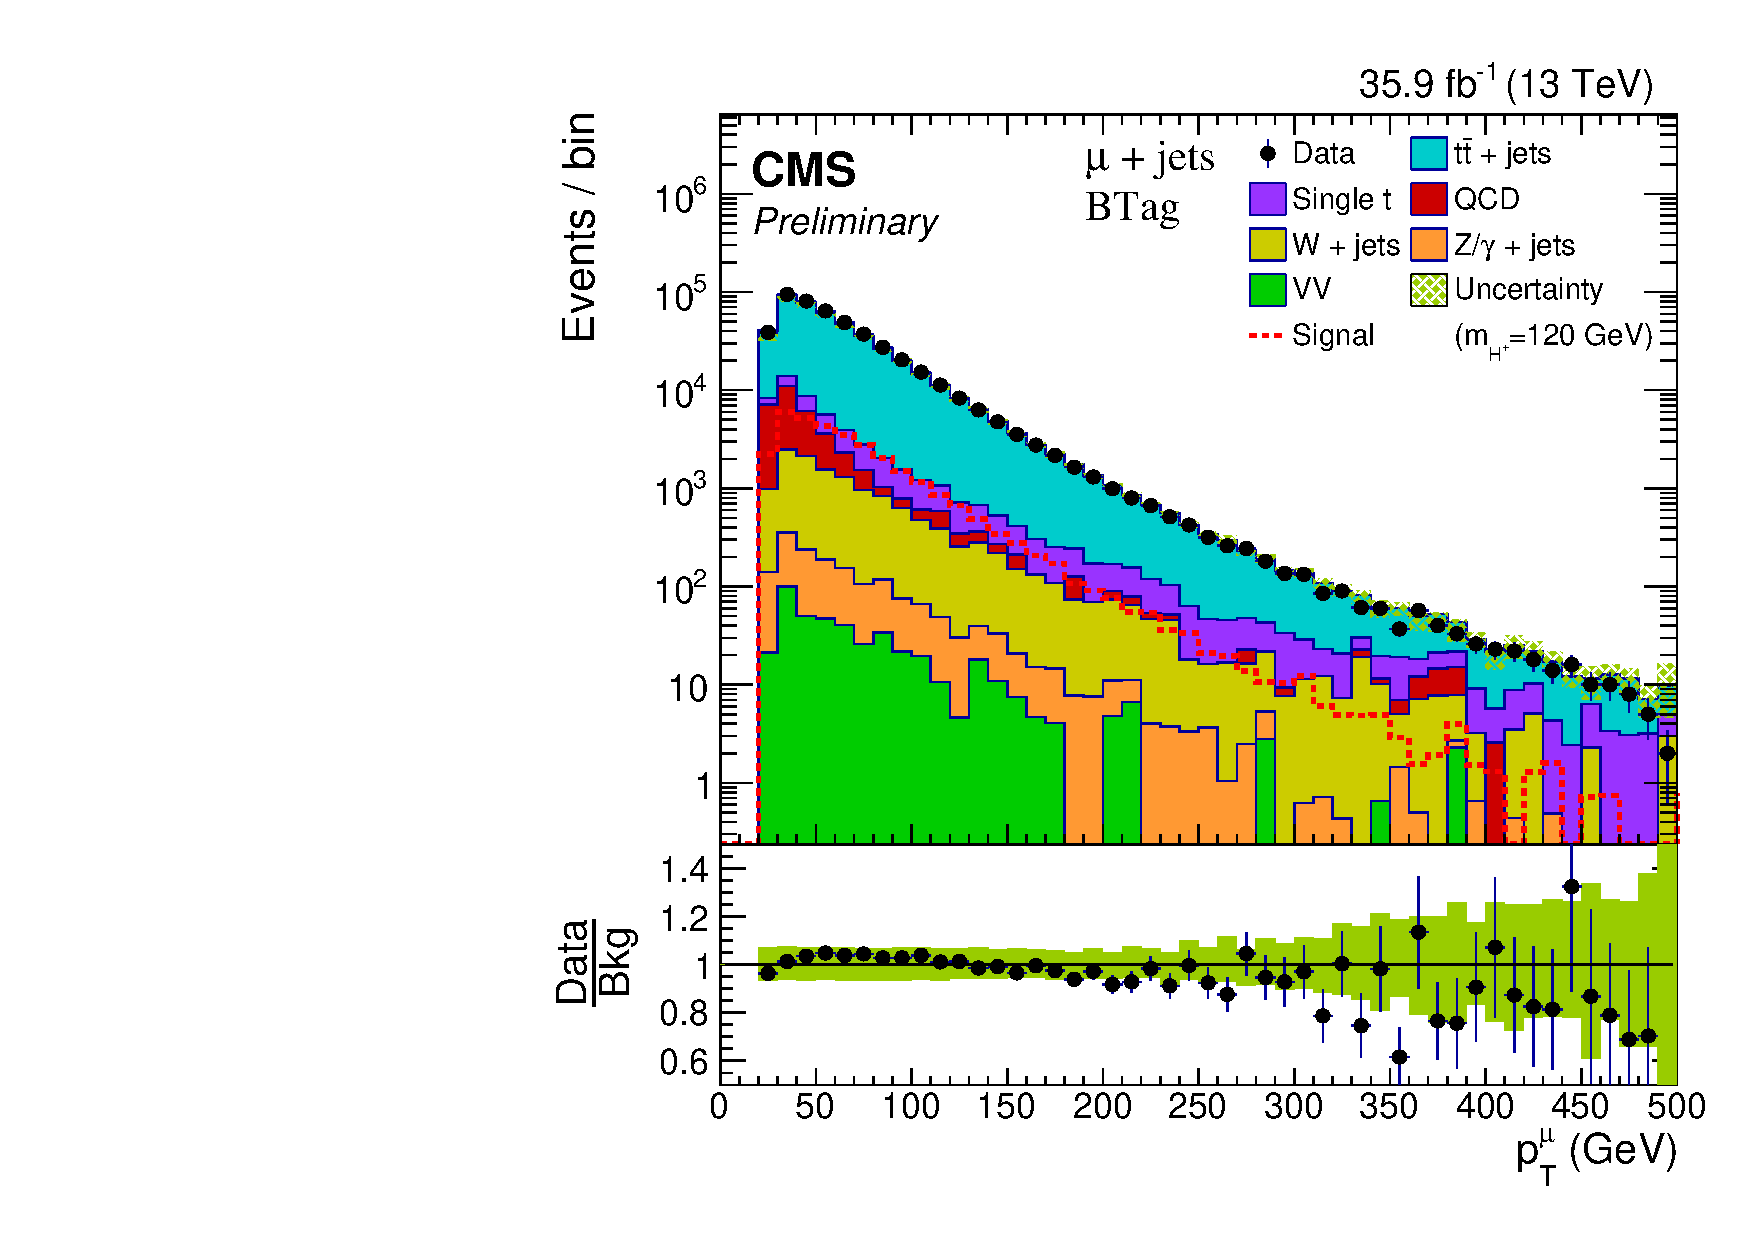
\includegraphics[width=0.40\linewidth]{Image/Muon/BTag/pt_mu_muBTag.pdf}}
    \subfigure[\pt of electron]{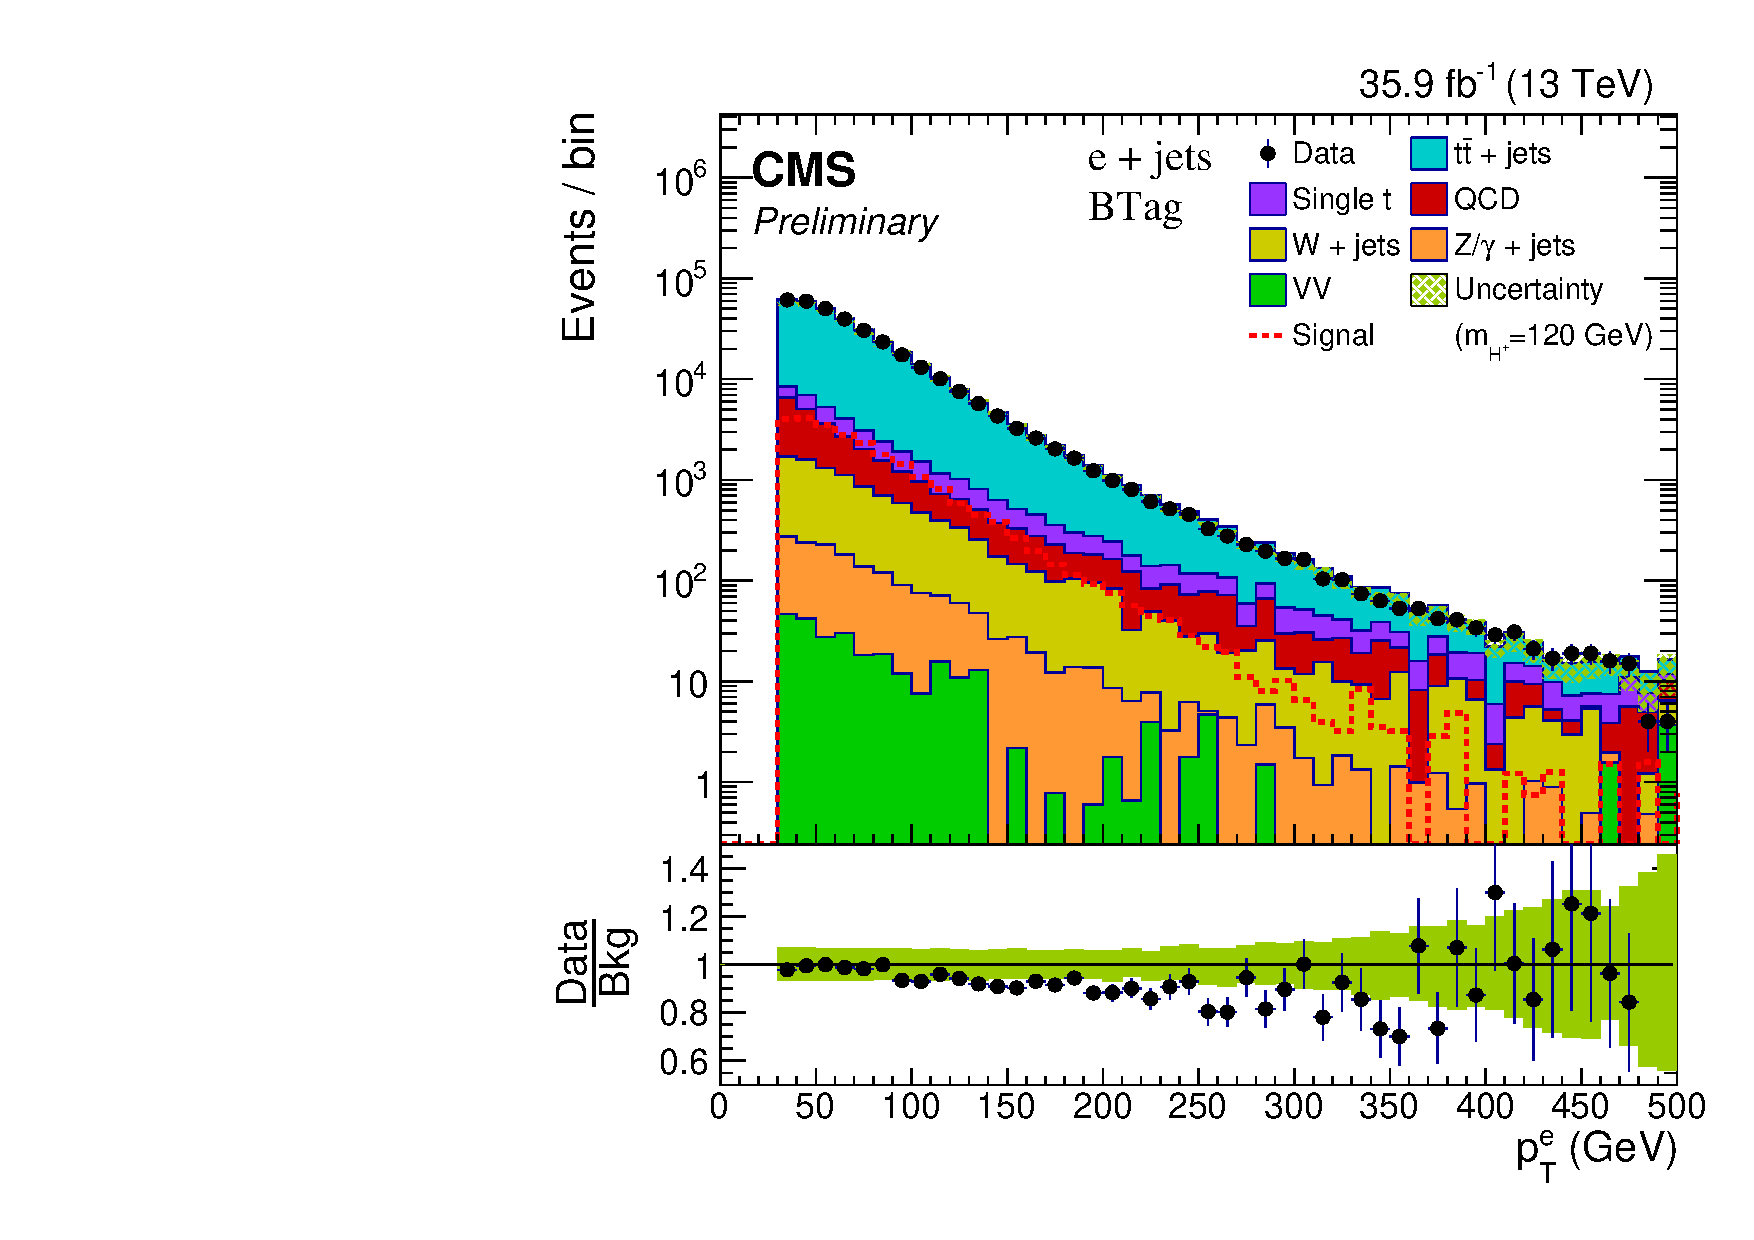
\includegraphics[width=0.40\linewidth]{Image/Electron/BTag/pt_ele_eleBTag.pdf}}
    \vfil
    \subfigure[$\eta$ of muon]{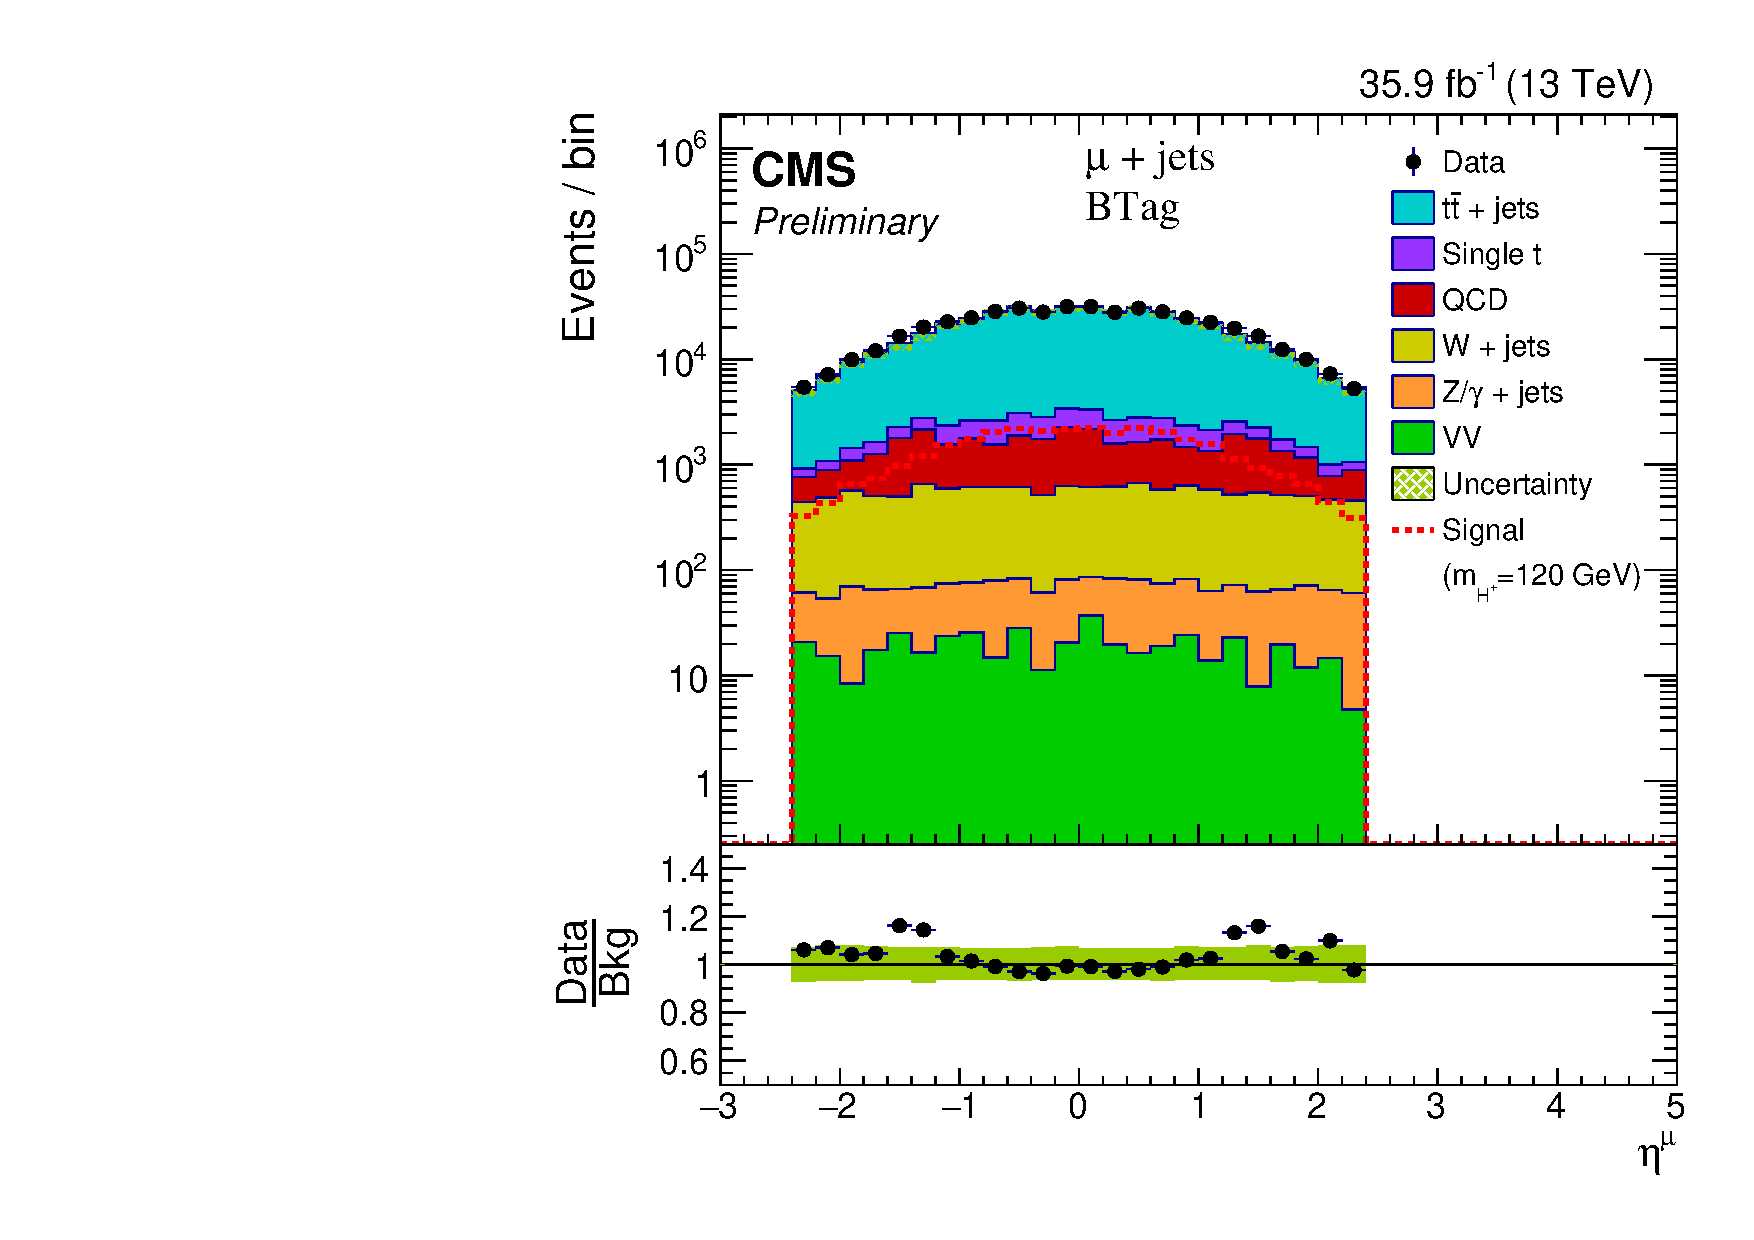
\includegraphics[width=0.40\linewidth]{Image/Muon/BTag/eta_mu_muBTag.pdf}}
    \subfigure[$\eta$ of electron]{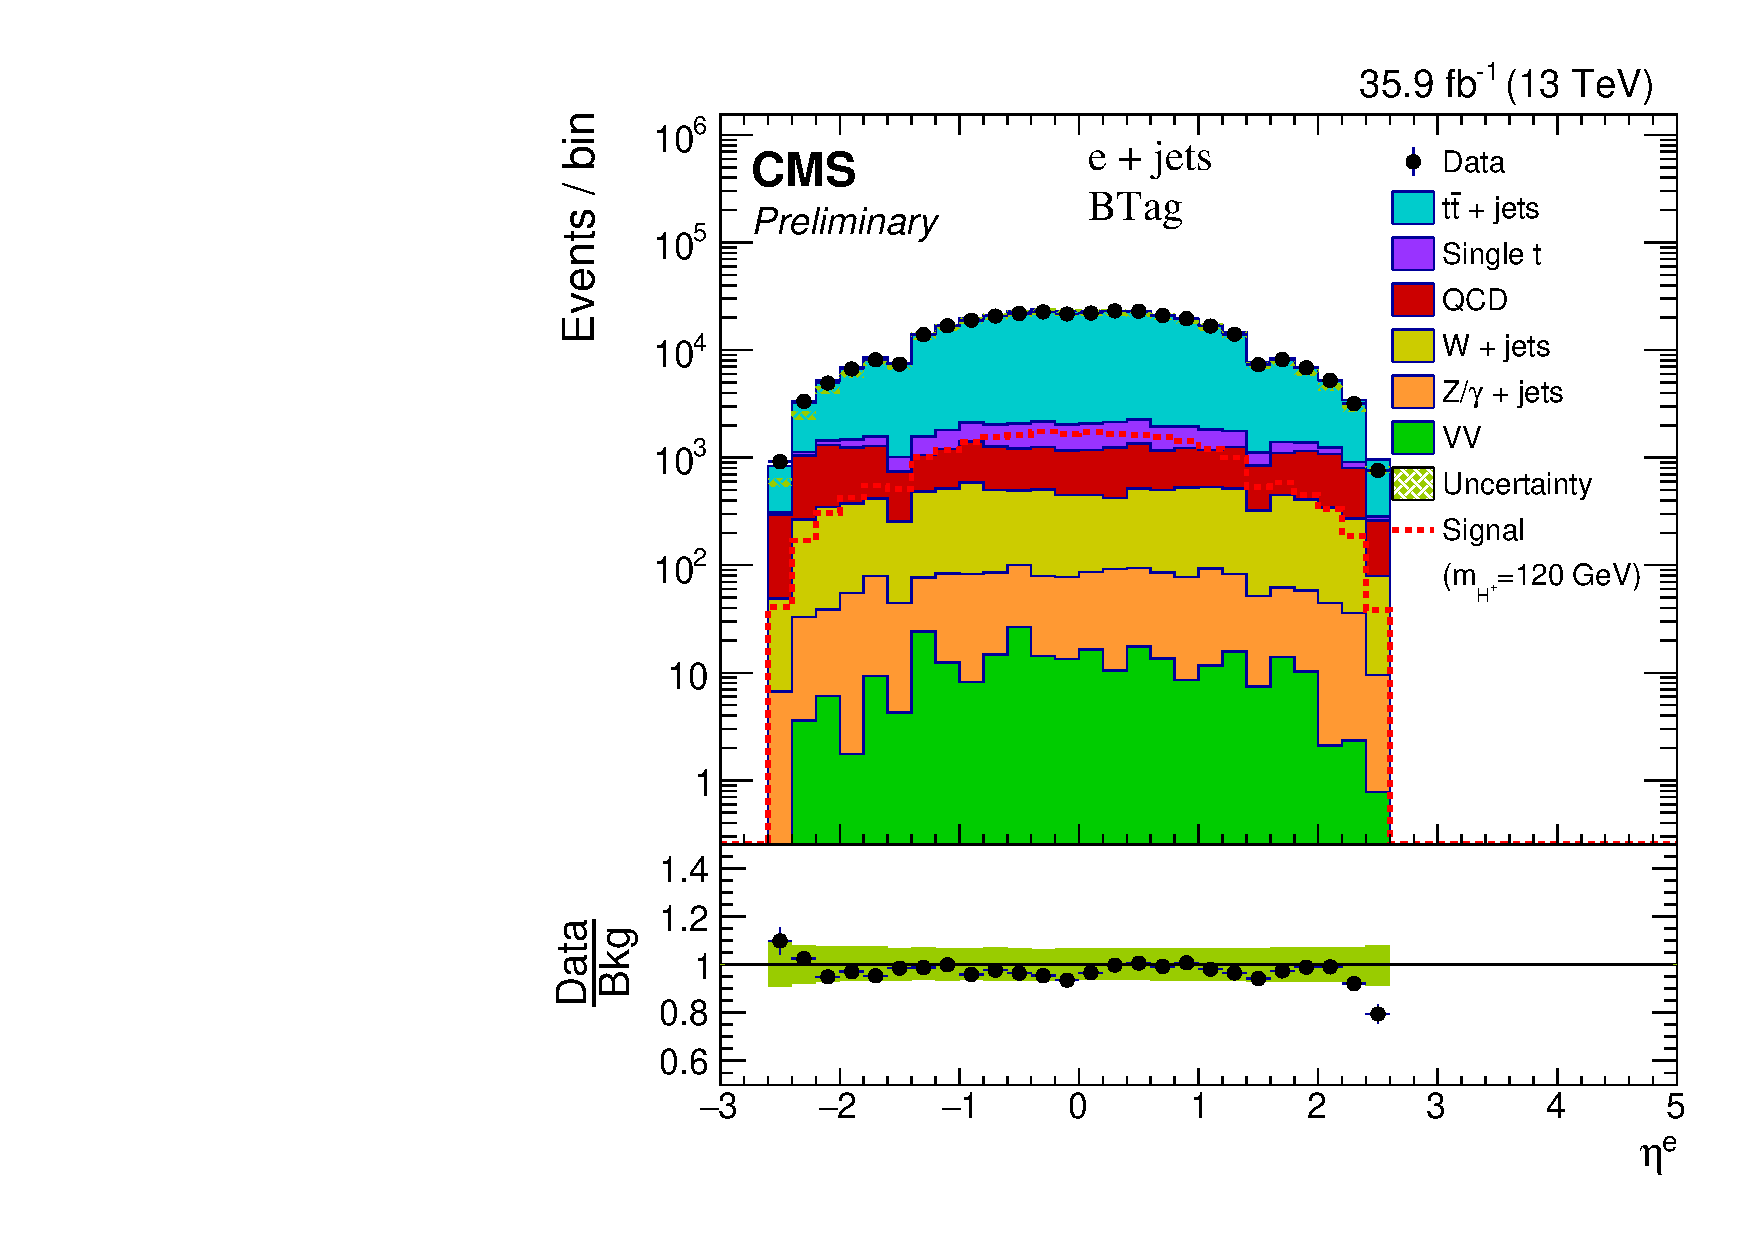
\includegraphics[width=0.40\linewidth]{Image/Electron/BTag/eta_ele_eleBTag.pdf}}
    \vfil
    \subfigure[\pt of jets]{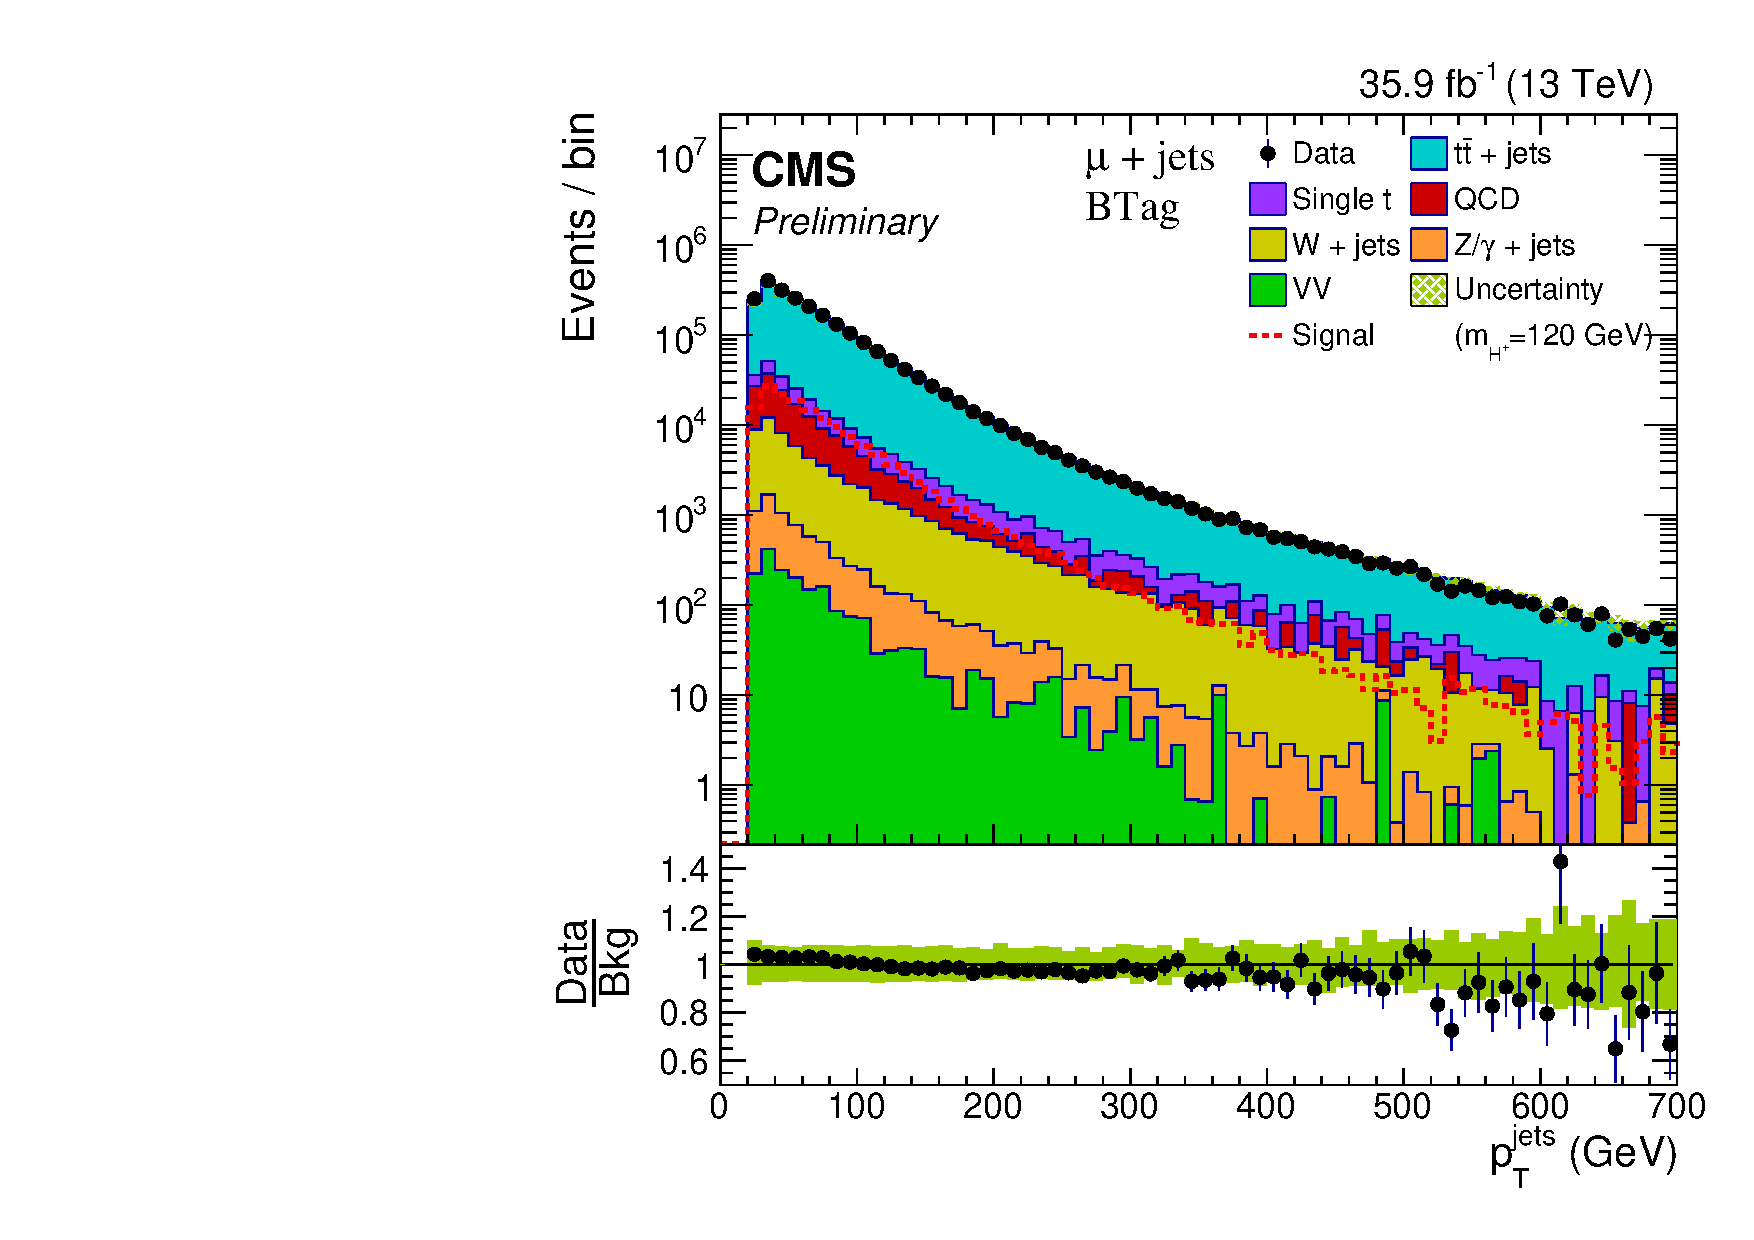
\includegraphics[width=0.40\linewidth]{Image/Muon/BTag/pt_jet_muBTag.pdf}}
    \subfigure[\pt of jets]{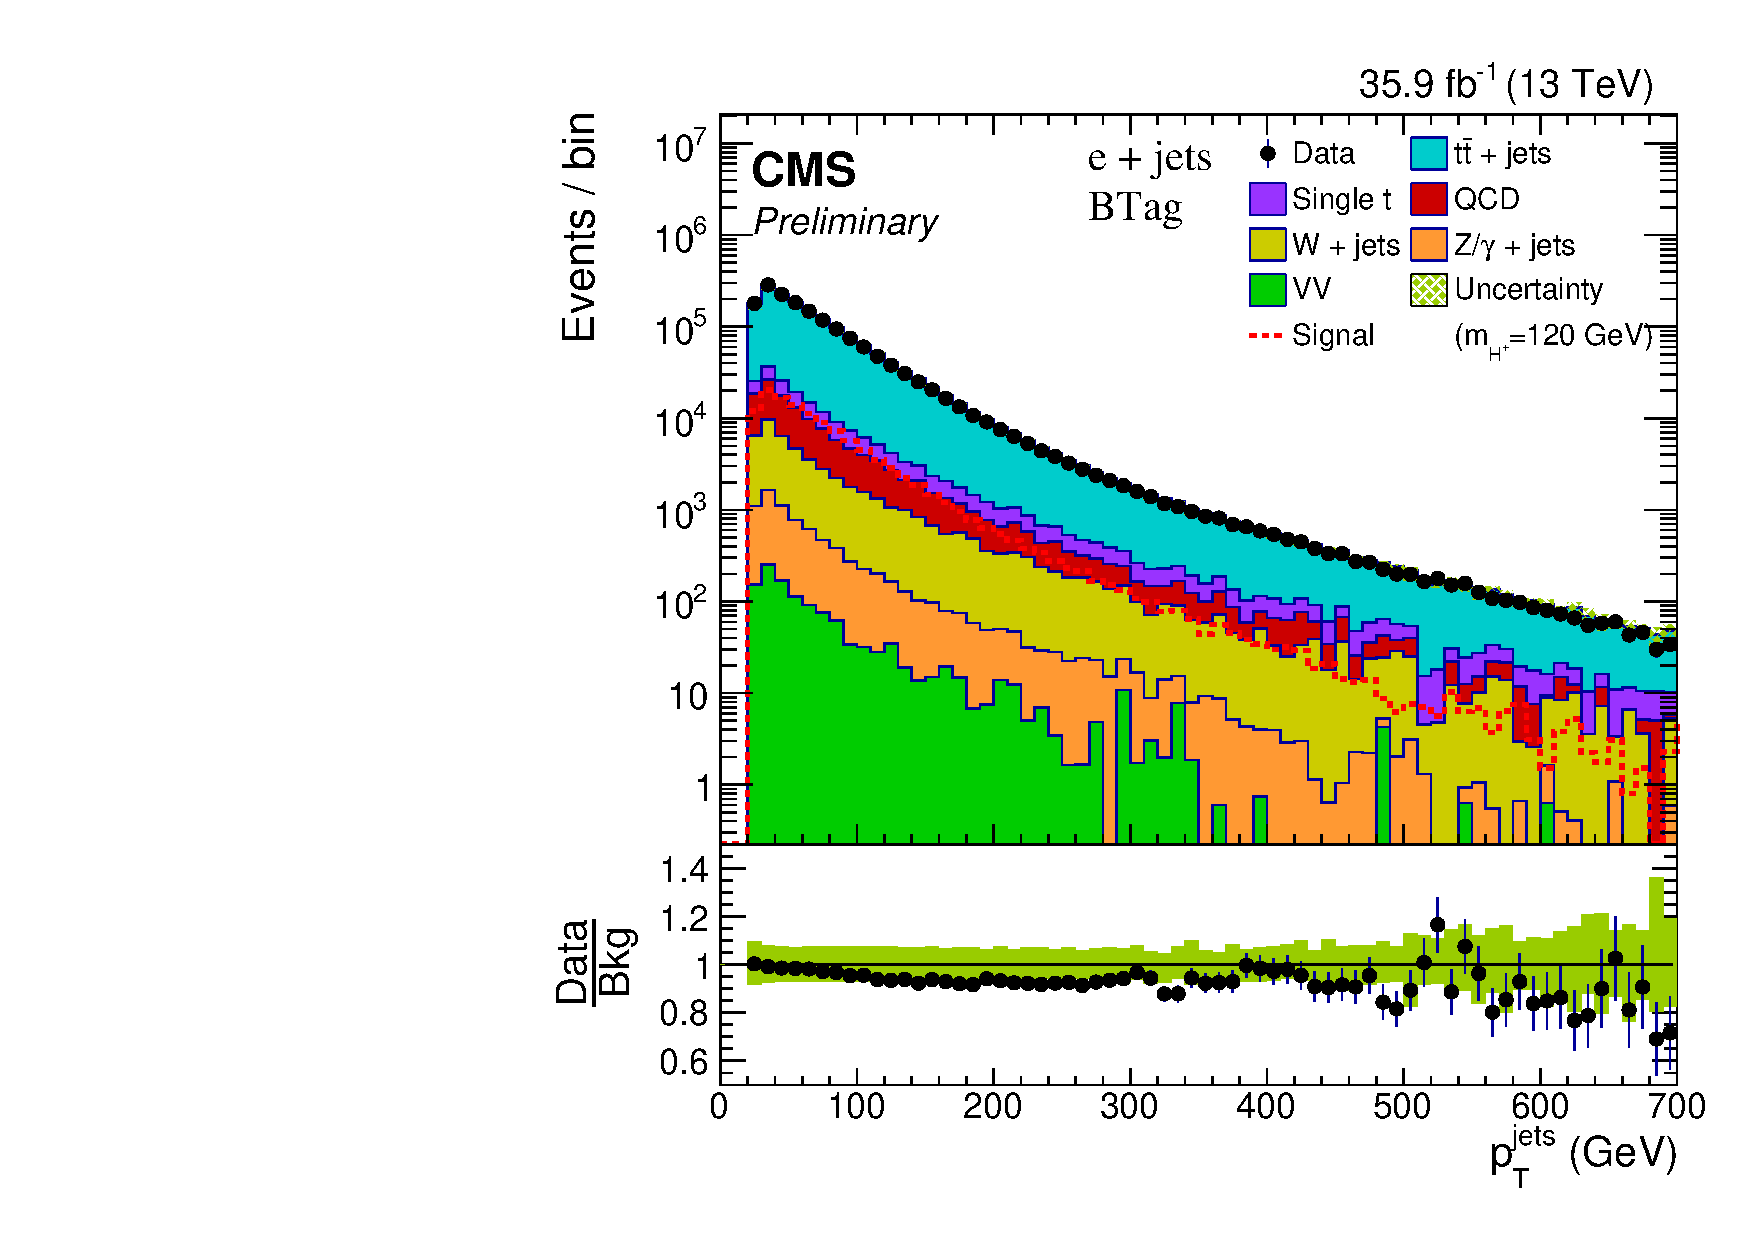
\includegraphics[width=0.40\linewidth]{Image/Electron/BTag/pt_jet_eleBTag.pdf}}
    \caption{Distribution of $\pt, \eta$ of reconstructed lepton and \pt of jets
        after \PQb jet selection as described in Section~\ref{s:secEvtSel}, 
    for \mujets and \ejets channel.}
    \label{fig:btagPlot1}
\end{figure}

%After BTagging: Eta_jets, N_jets, N_bjets
\begin{figure}
    \centering  
    \subfigure[$\eta$ of jets]{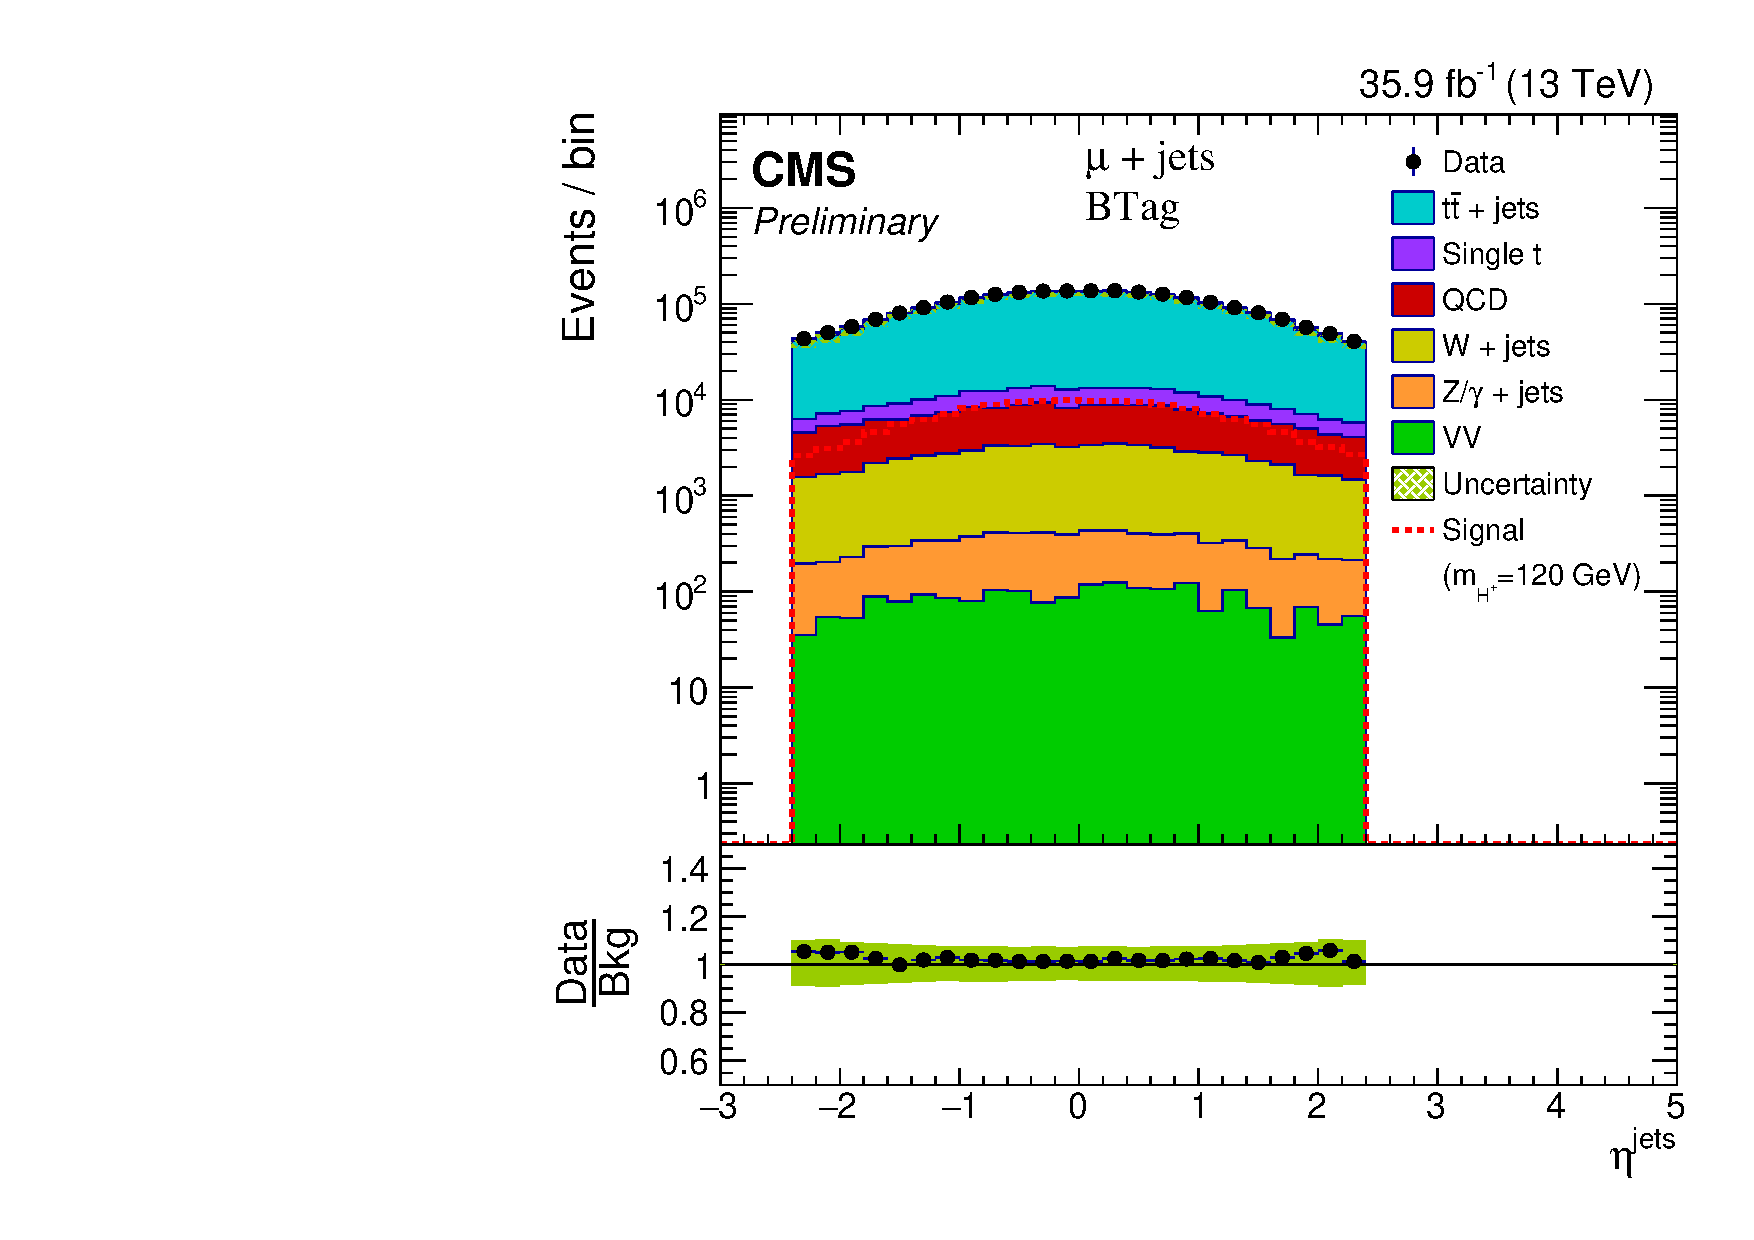
\includegraphics[width=0.40\linewidth]{Image/Muon/BTag/eta_jet_muBTag.pdf}}
    \subfigure[$\eta$ of jets]{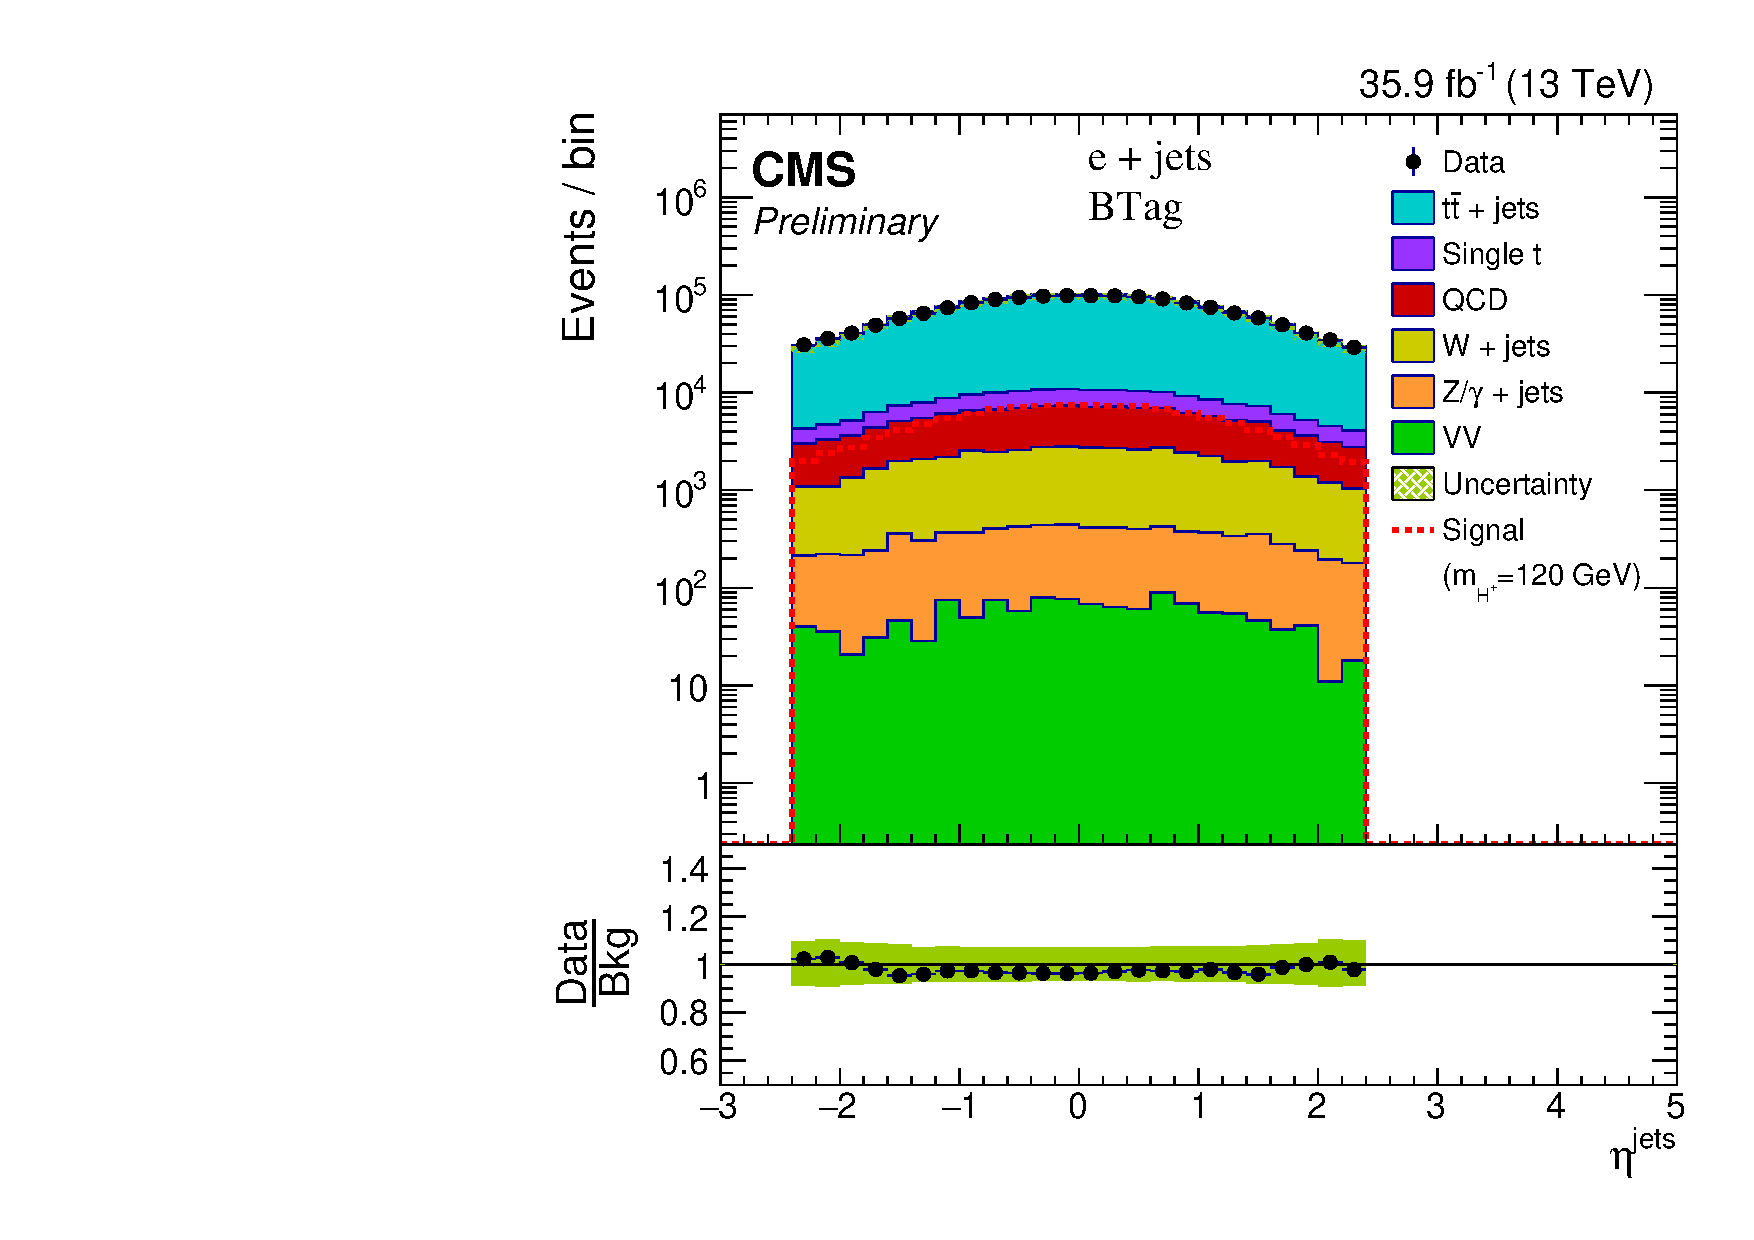
\includegraphics[width=0.40\linewidth]{Image/Electron/BTag/eta_jet_eleBTag.pdf}}
    \vfil
    \subfigure[jet multiplicity]{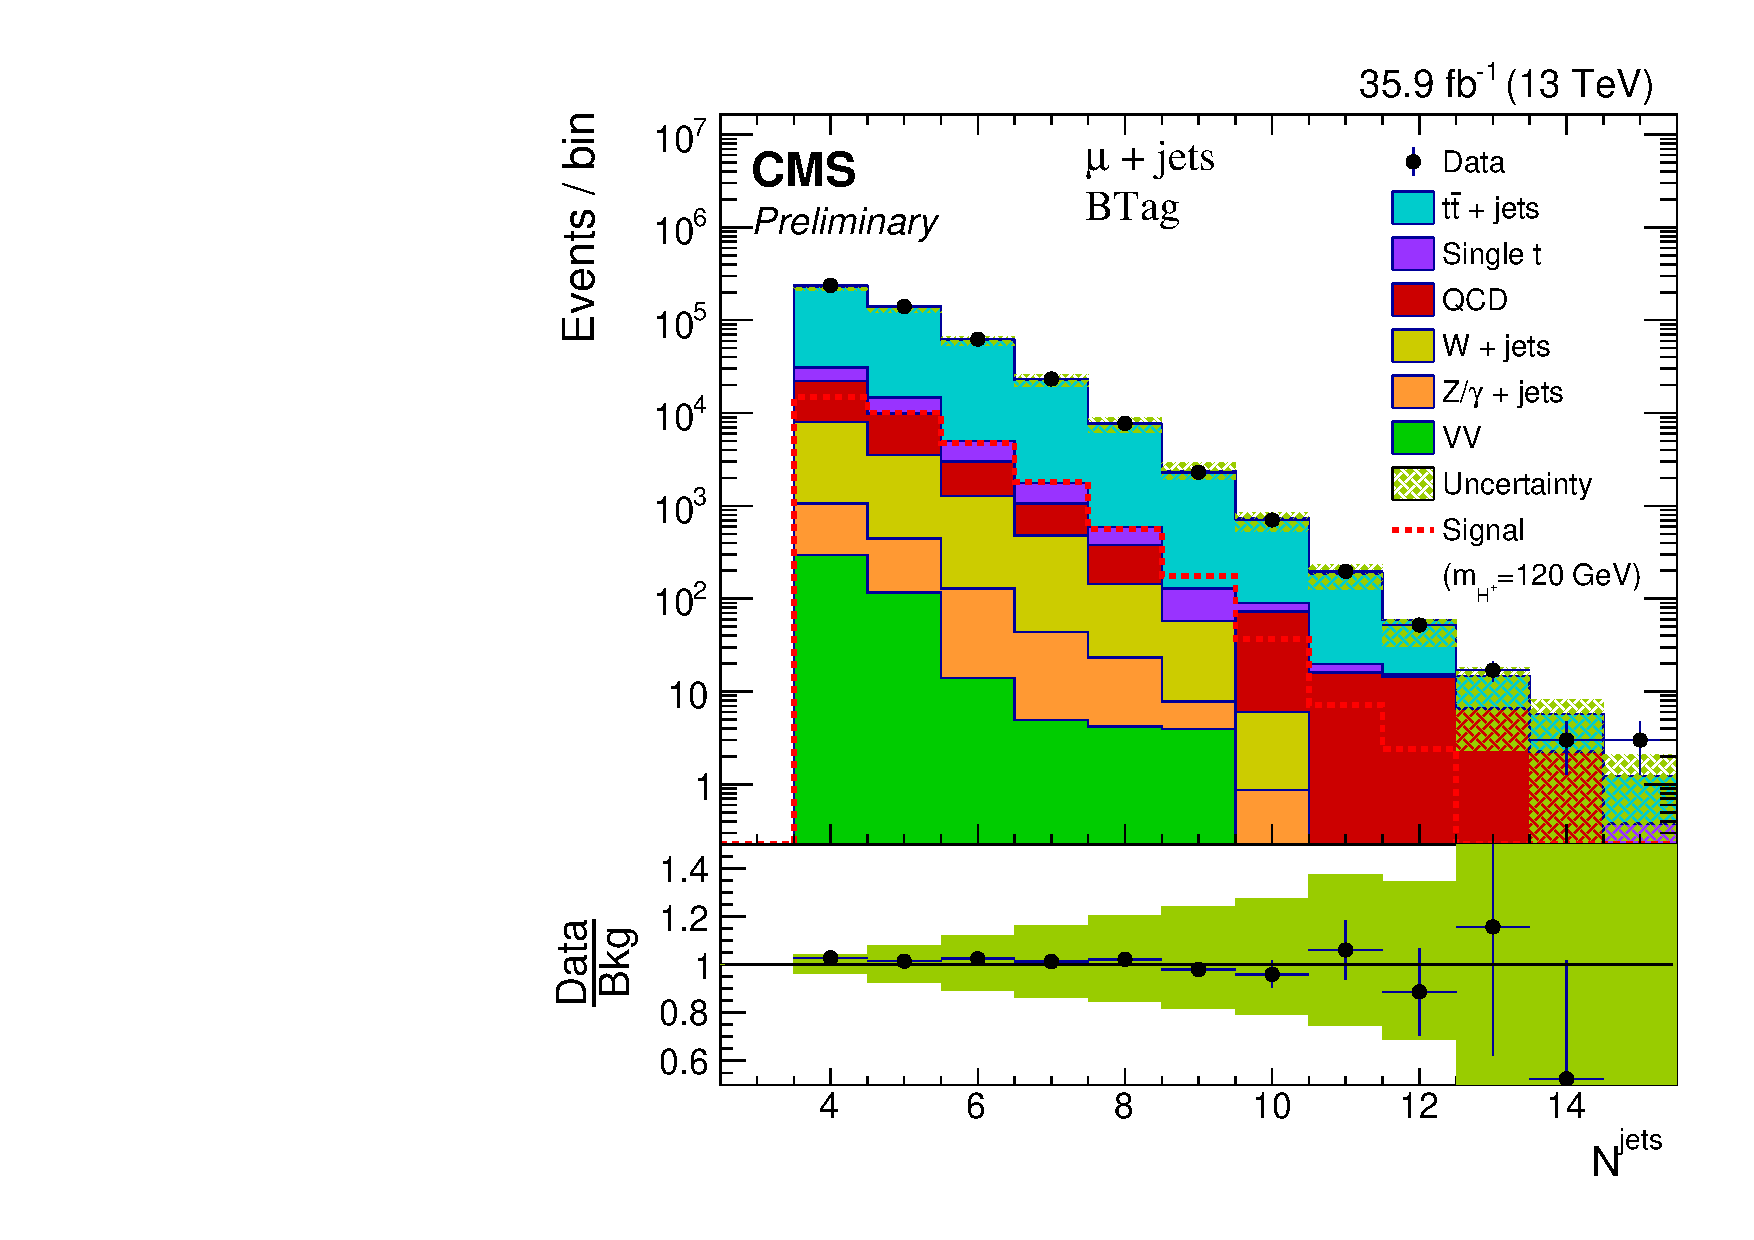
\includegraphics[width=0.40\linewidth]{Image/Muon/BTag/final_multi_jet_muBTag.pdf}}
    \subfigure[jet multiplicity]{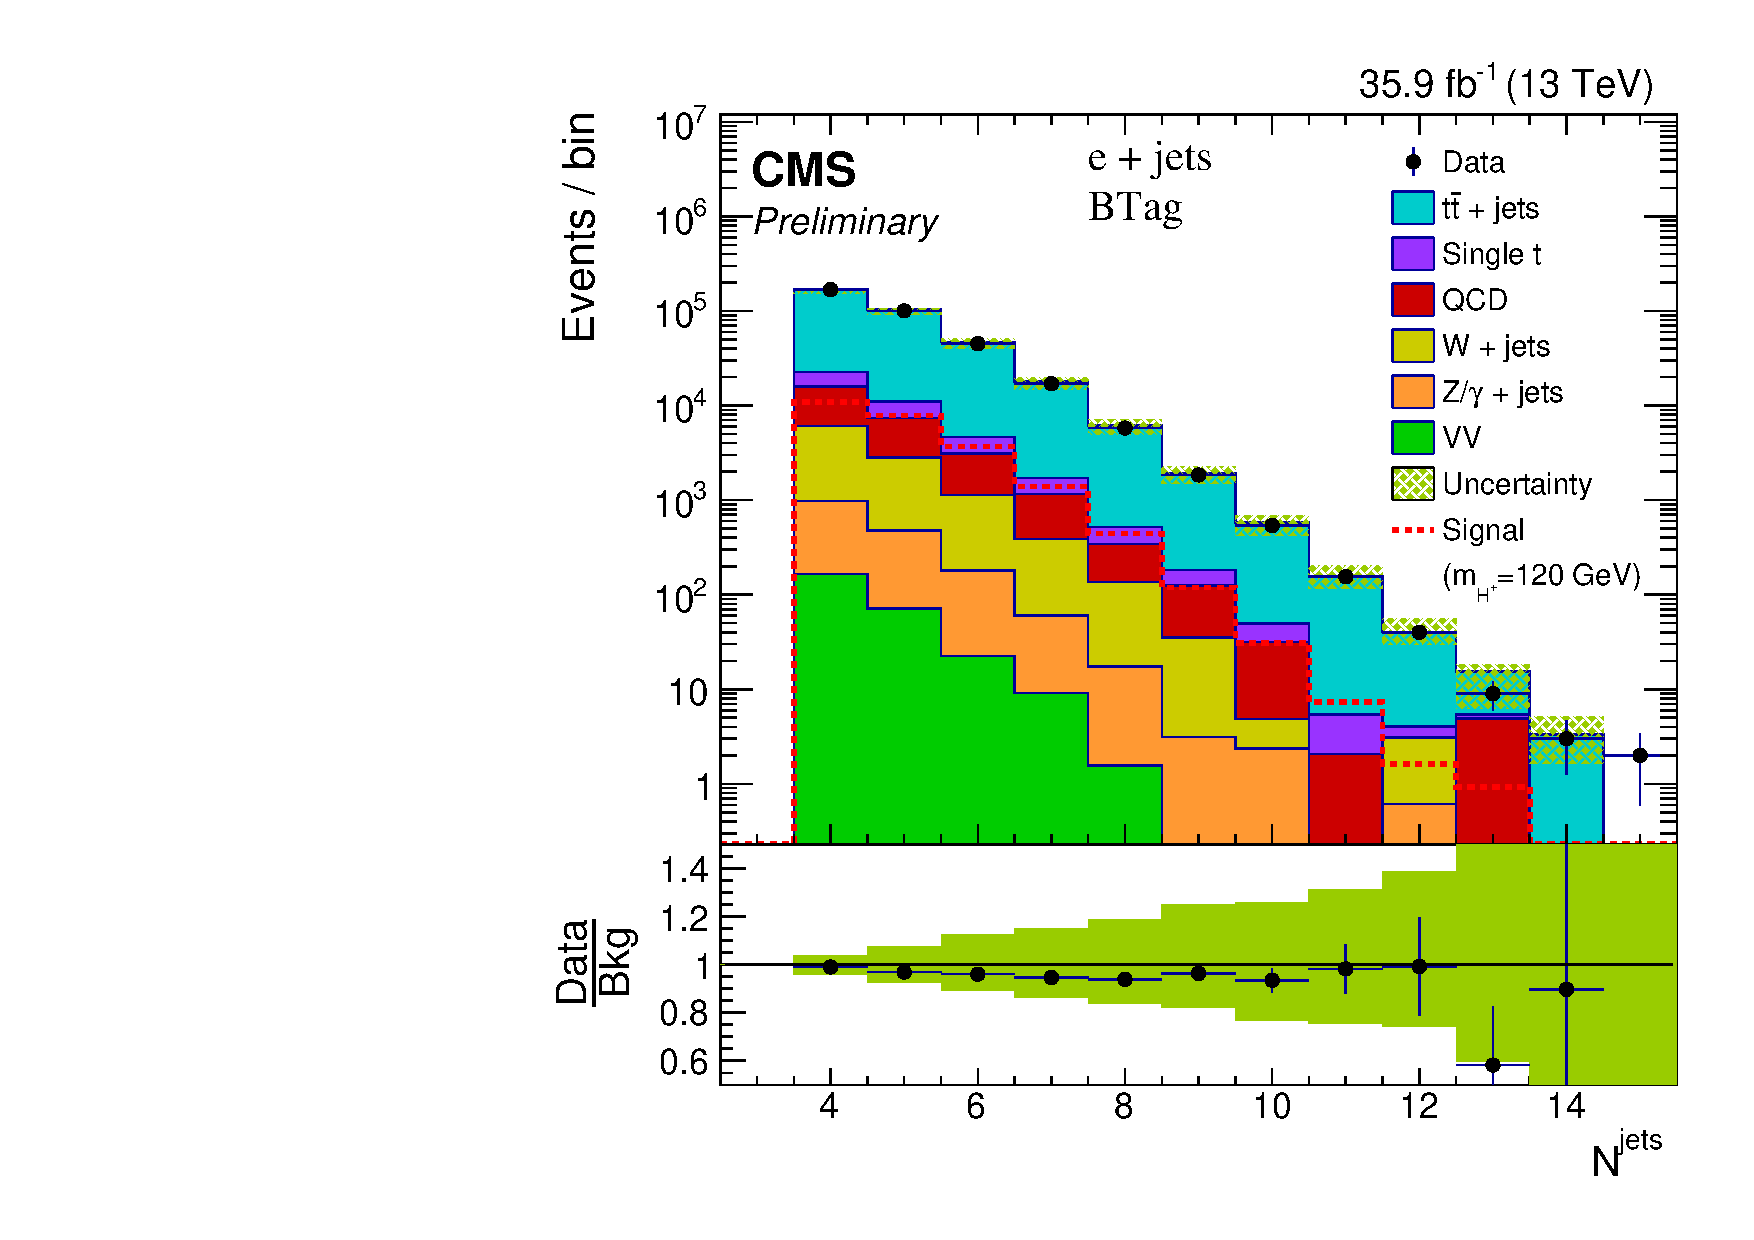
\includegraphics[width=0.40\linewidth]{Image/Electron/BTag/final_multi_jet_eleBTag.pdf}}
    \vfil
    \subfigure[\PQb jet multiplicity]{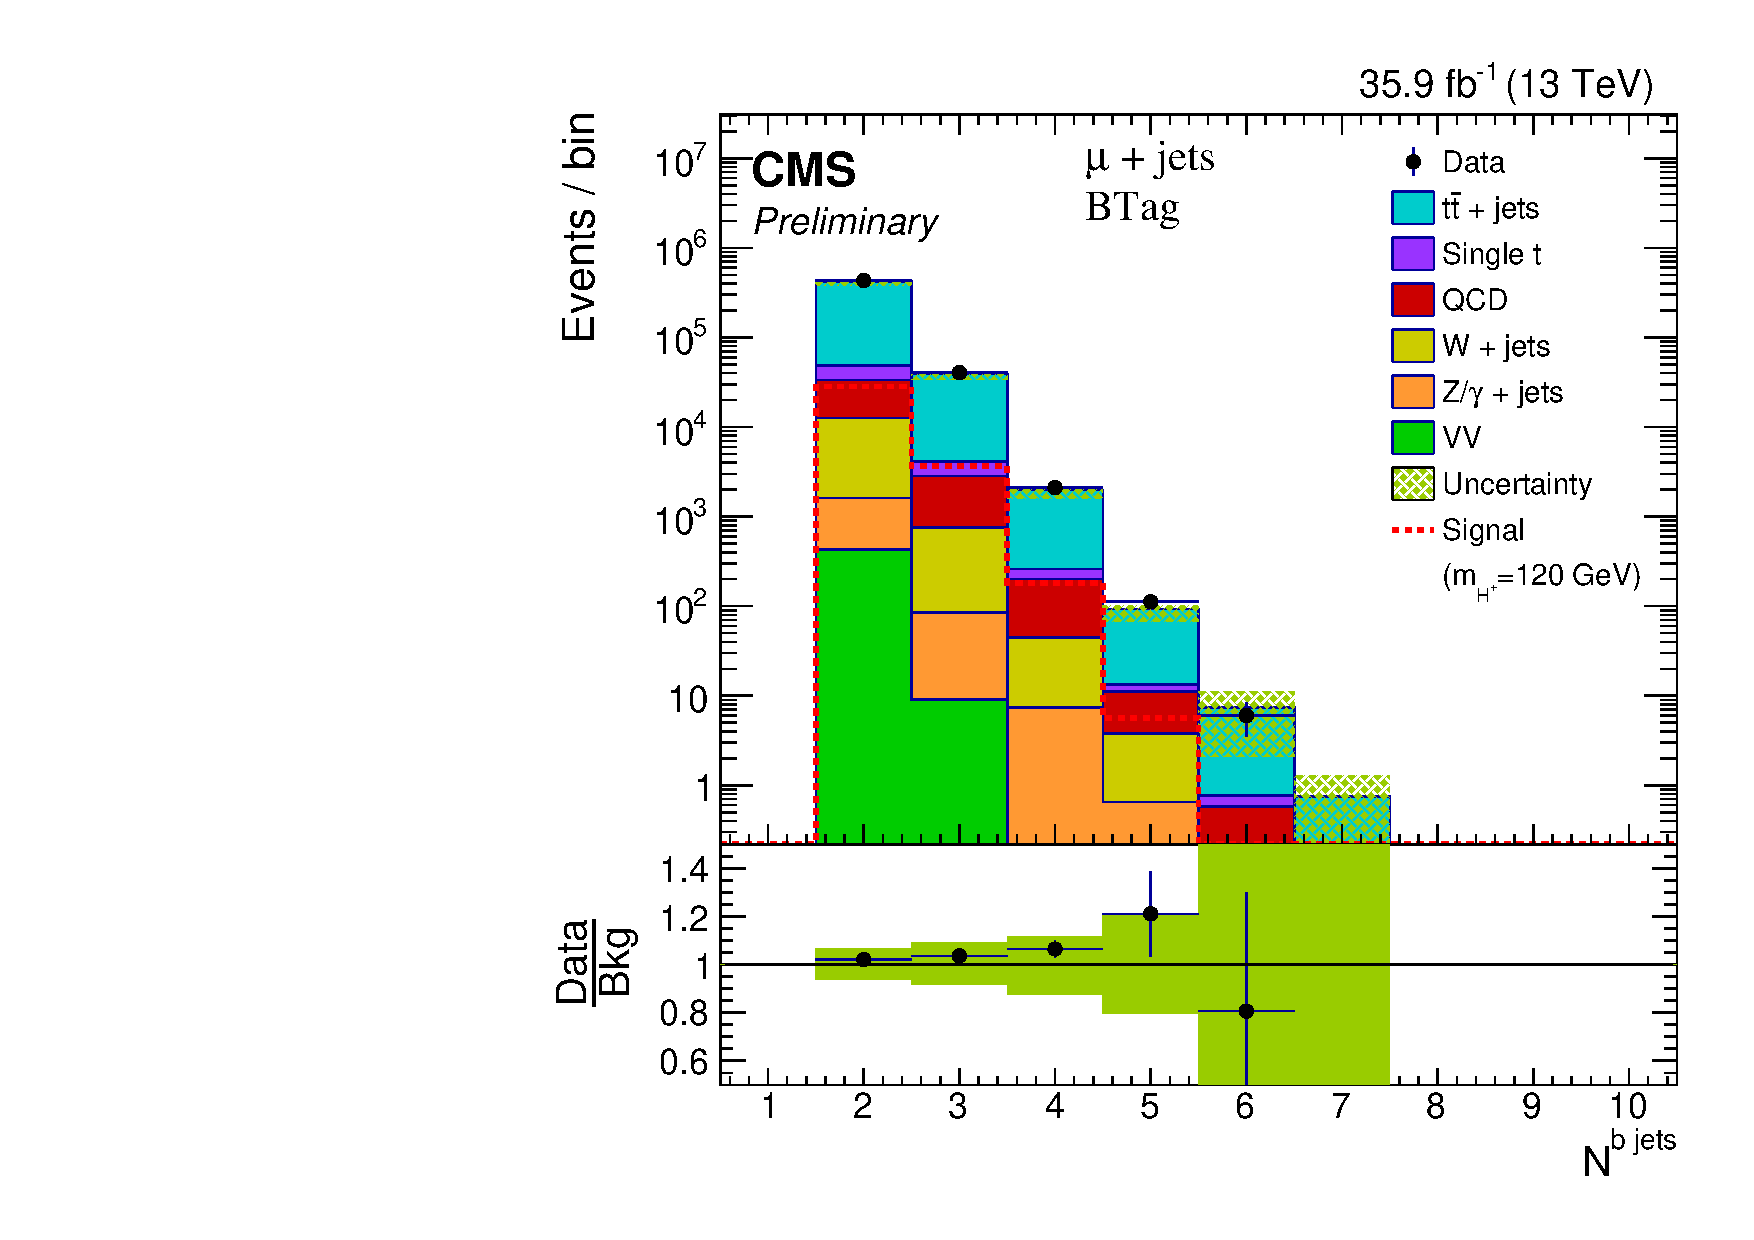
\includegraphics[width=0.40\linewidth]{Image/Muon/BTag/CSVL_count_muBTag.pdf}}
    \subfigure[\PQb jet multiplicity]{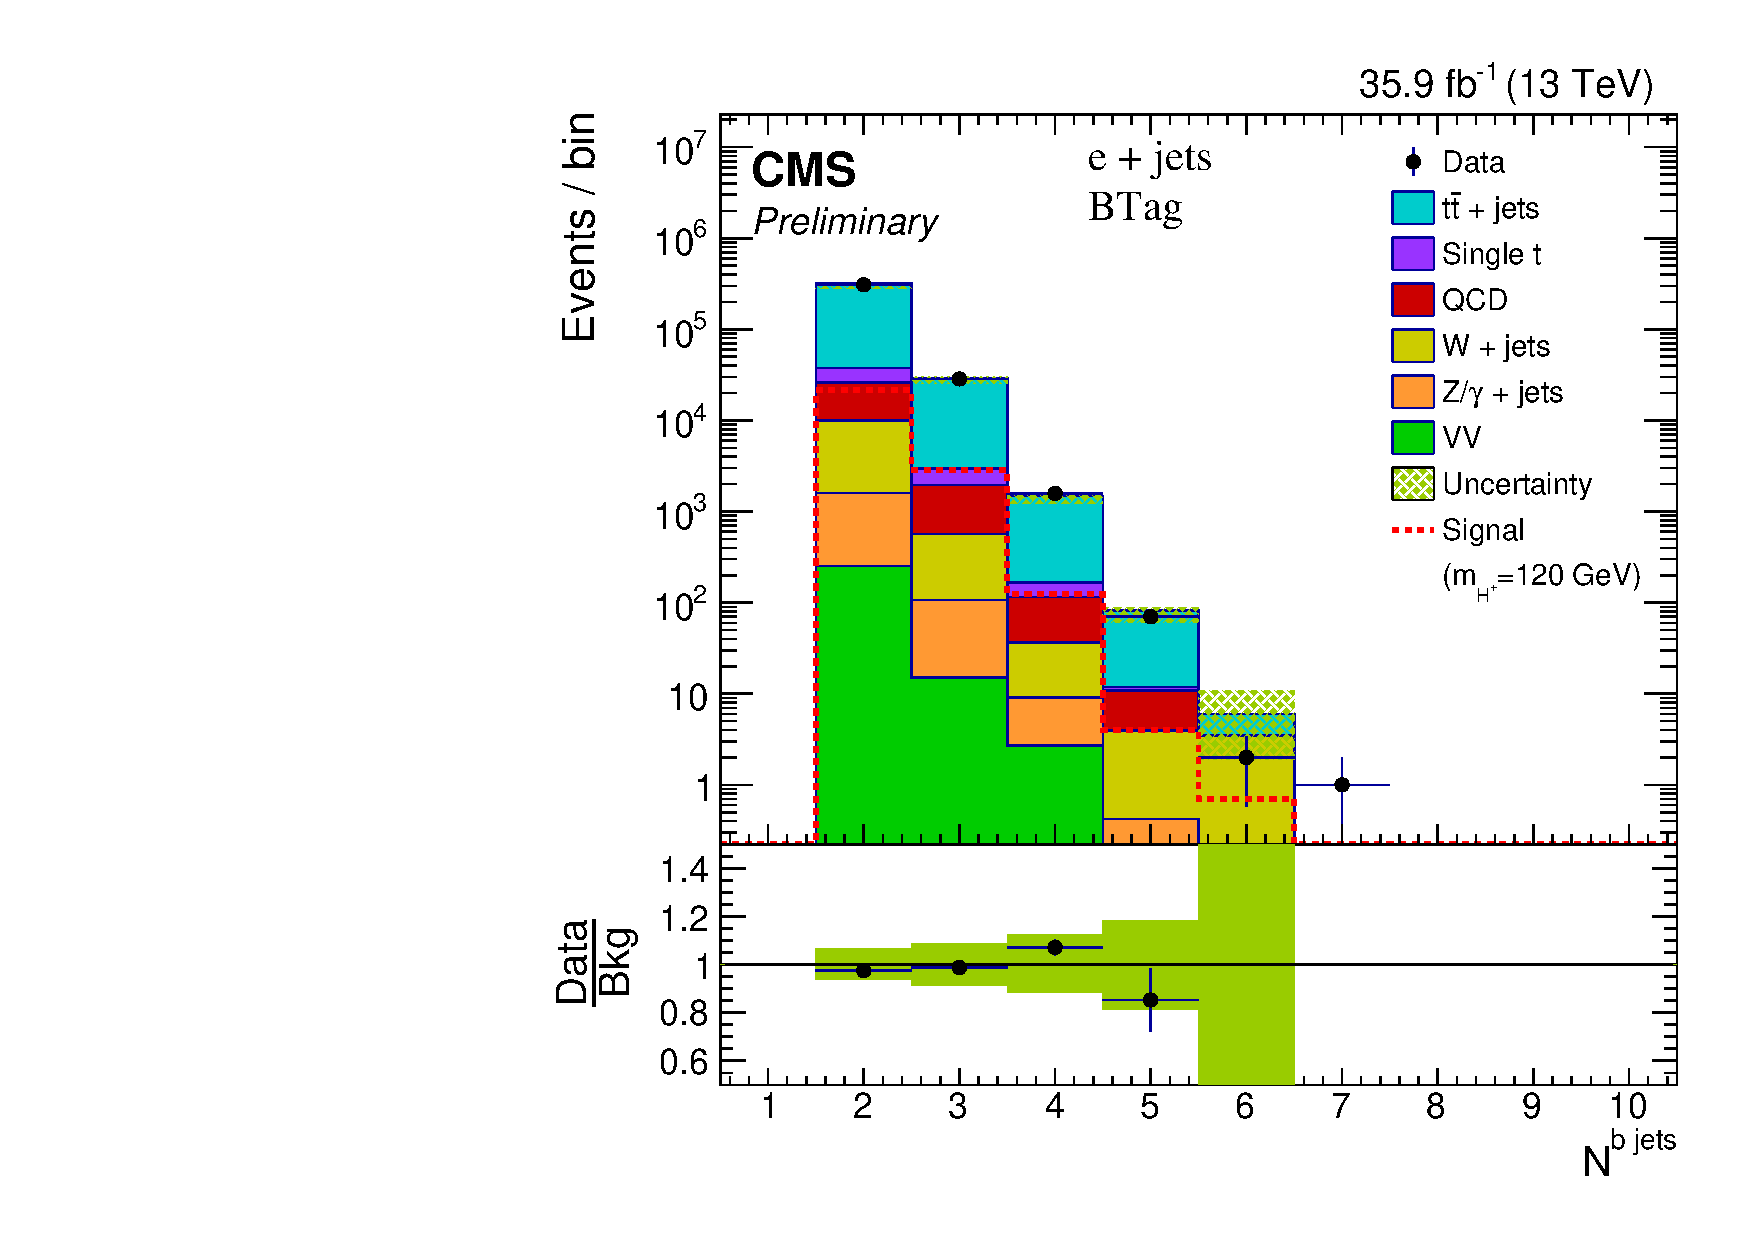
\includegraphics[width=0.40\linewidth]{Image/Electron/BTag/CSVL_count_eleBTag.pdf}}
    \caption{Distribution of reconstructed $\eta$ of jets, jet multiplicity, and 
        \PQb jet multiplicity after \PQb jet selection as described in 
        Section~\ref{s:secEvtSel}, for \mujets and \ejets channel.}
    \label{fig:btagPlot2}
\end{figure}

%After BTagging: \MET, MT 
\begin{figure}
    \centering  
    \subfigure[Missing transverse energy]{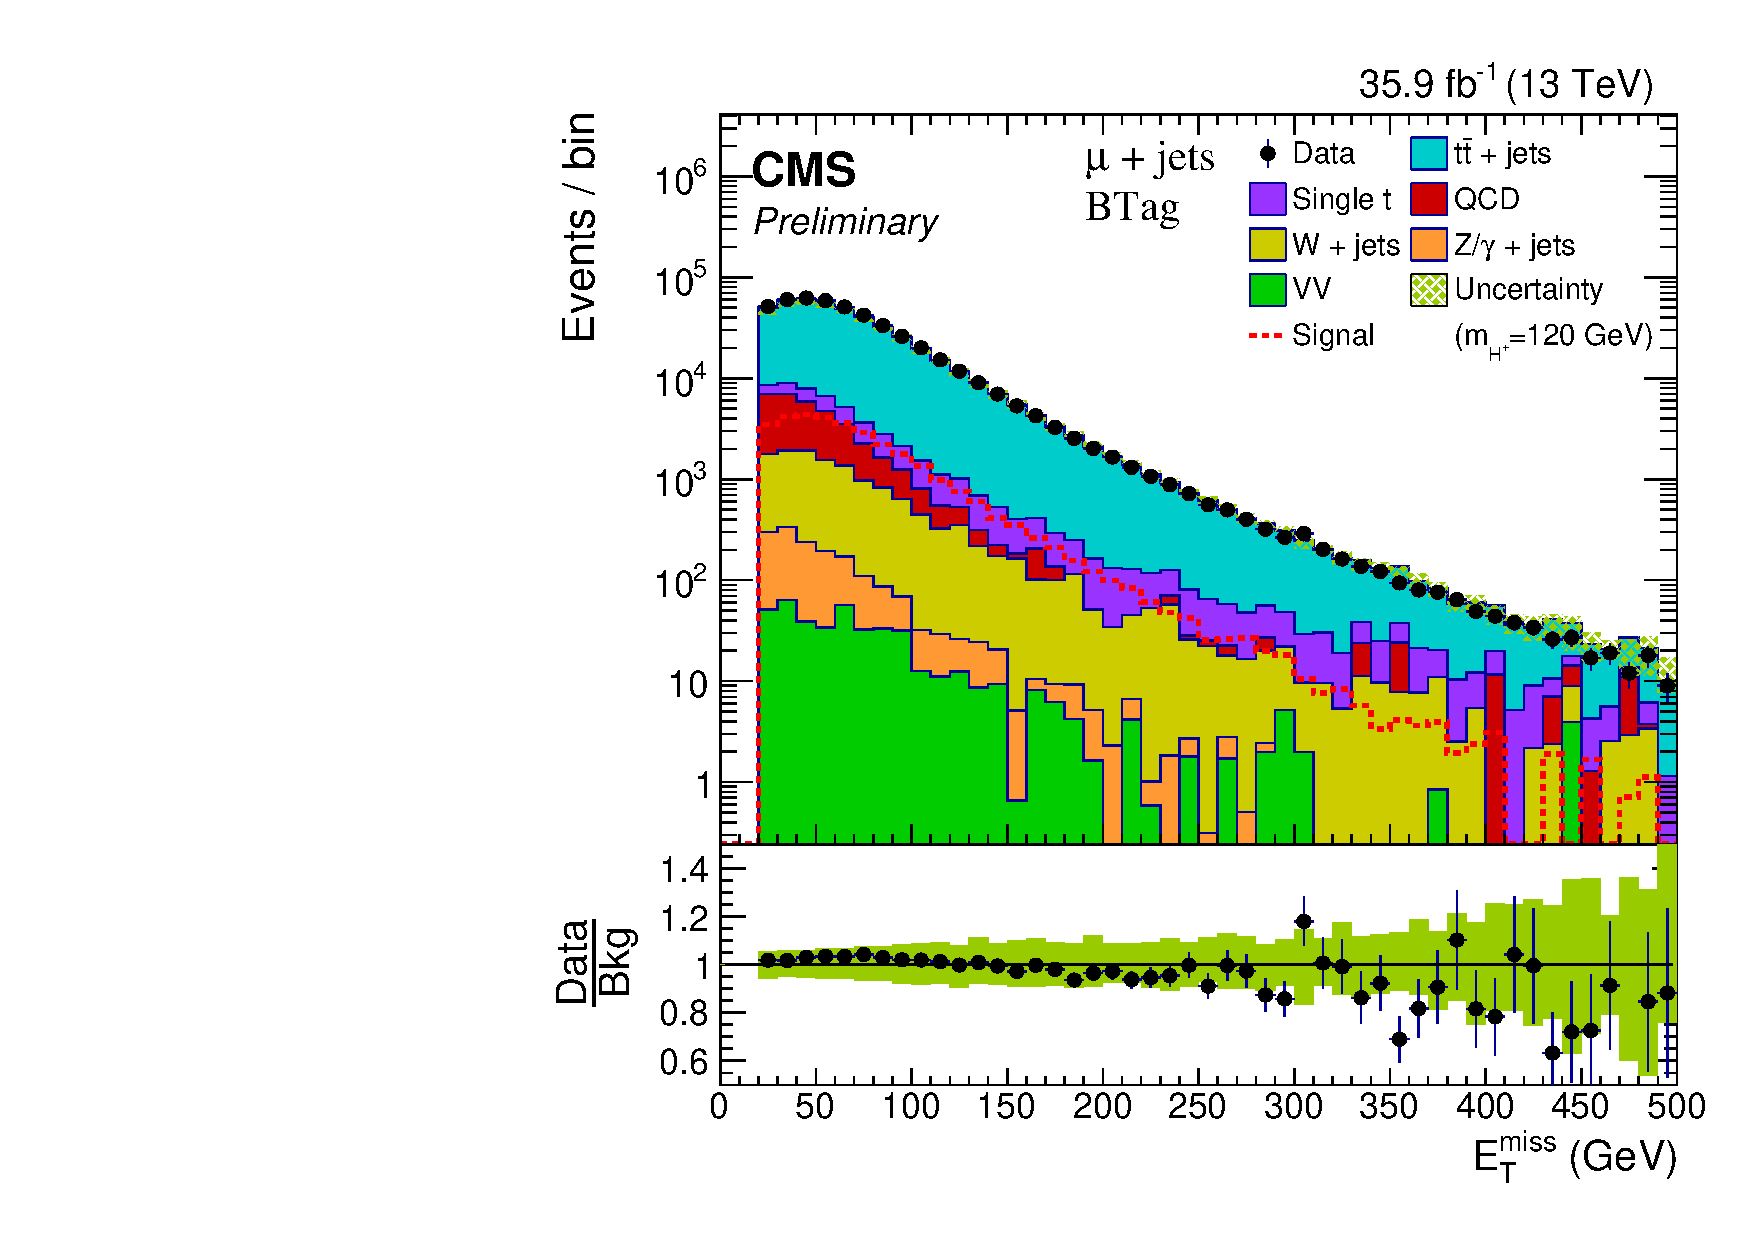
\includegraphics[width=0.45\linewidth]{Image/Muon/BTag/final_pt_met_muBTag.pdf}}
    \subfigure[Missing transverse energy]{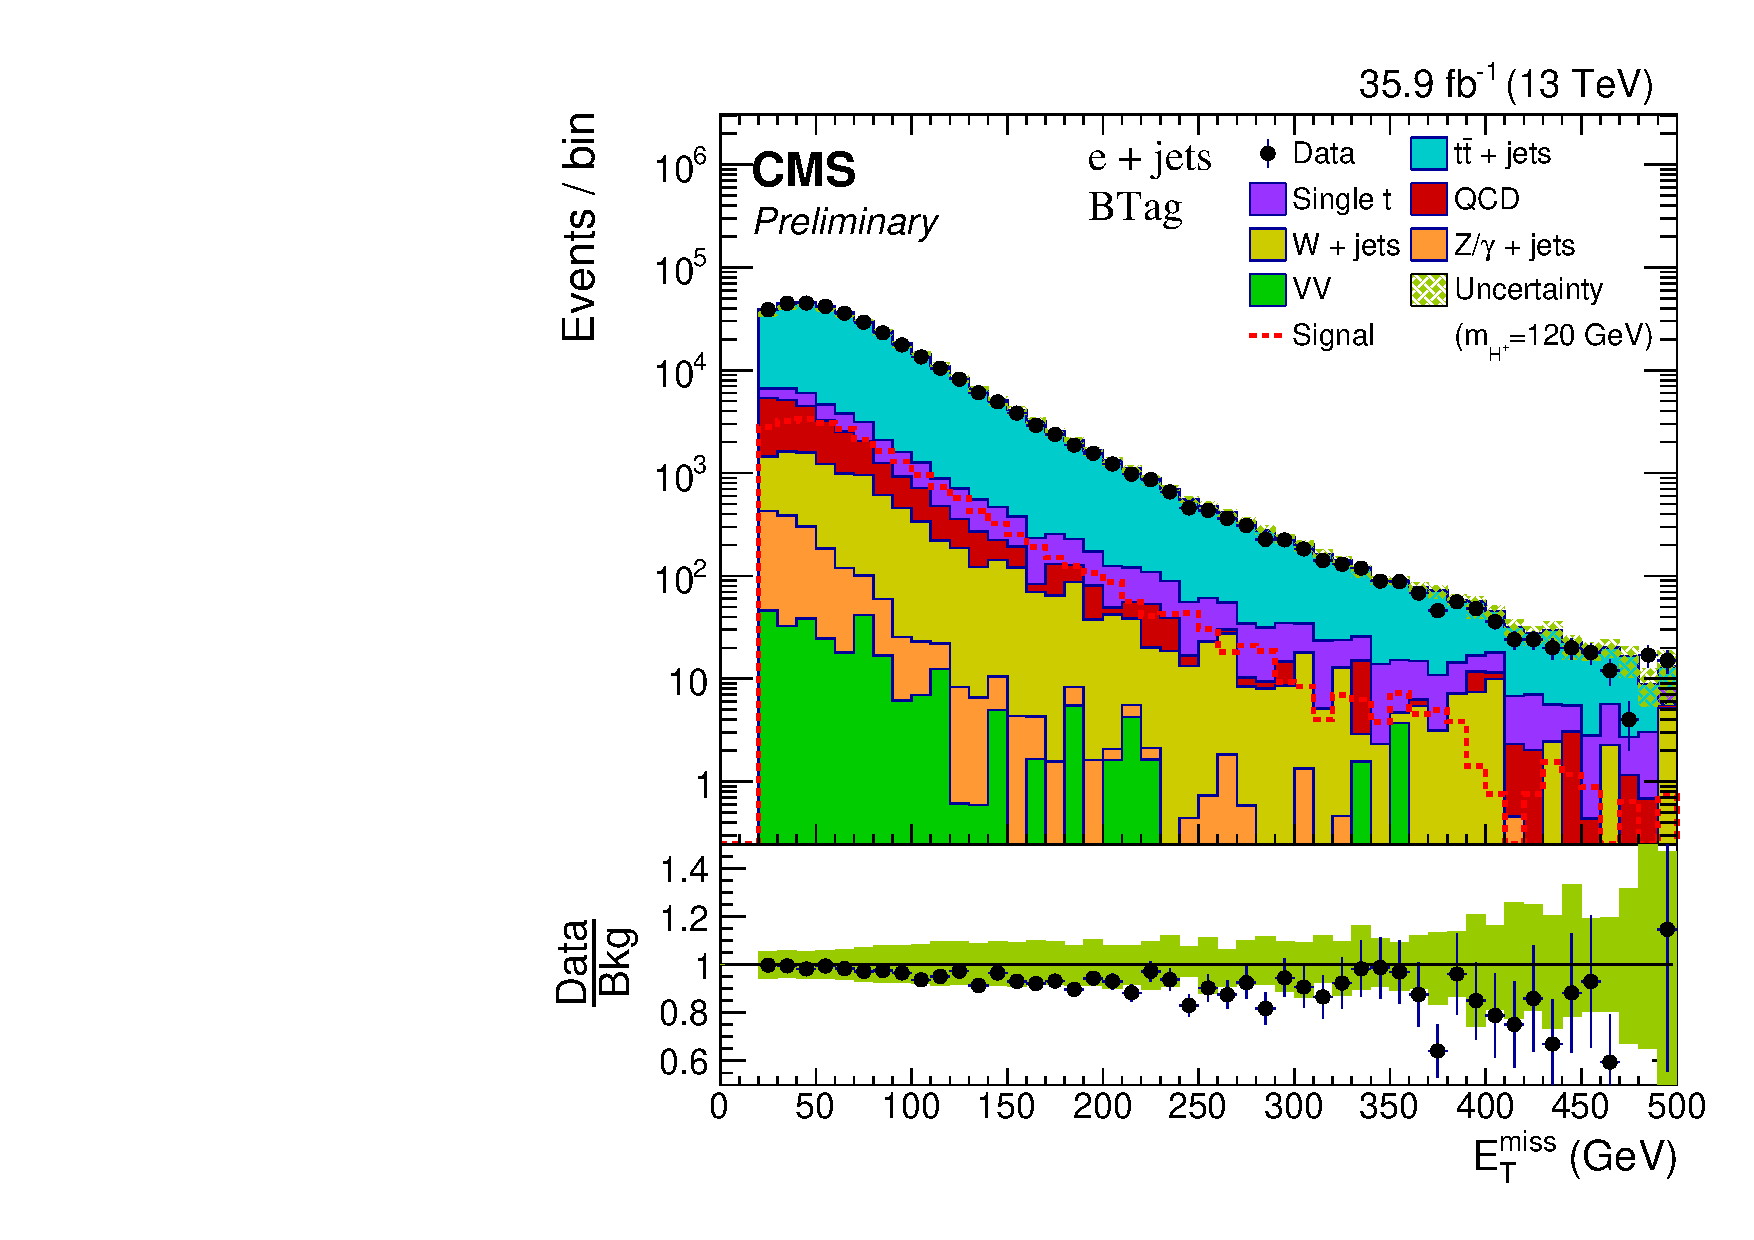
\includegraphics[width=0.45\linewidth]{Image/Electron/BTag/final_pt_met_eleBTag.pdf}}
    \vfil
    \subfigure[Transverse mass of \PW boson]{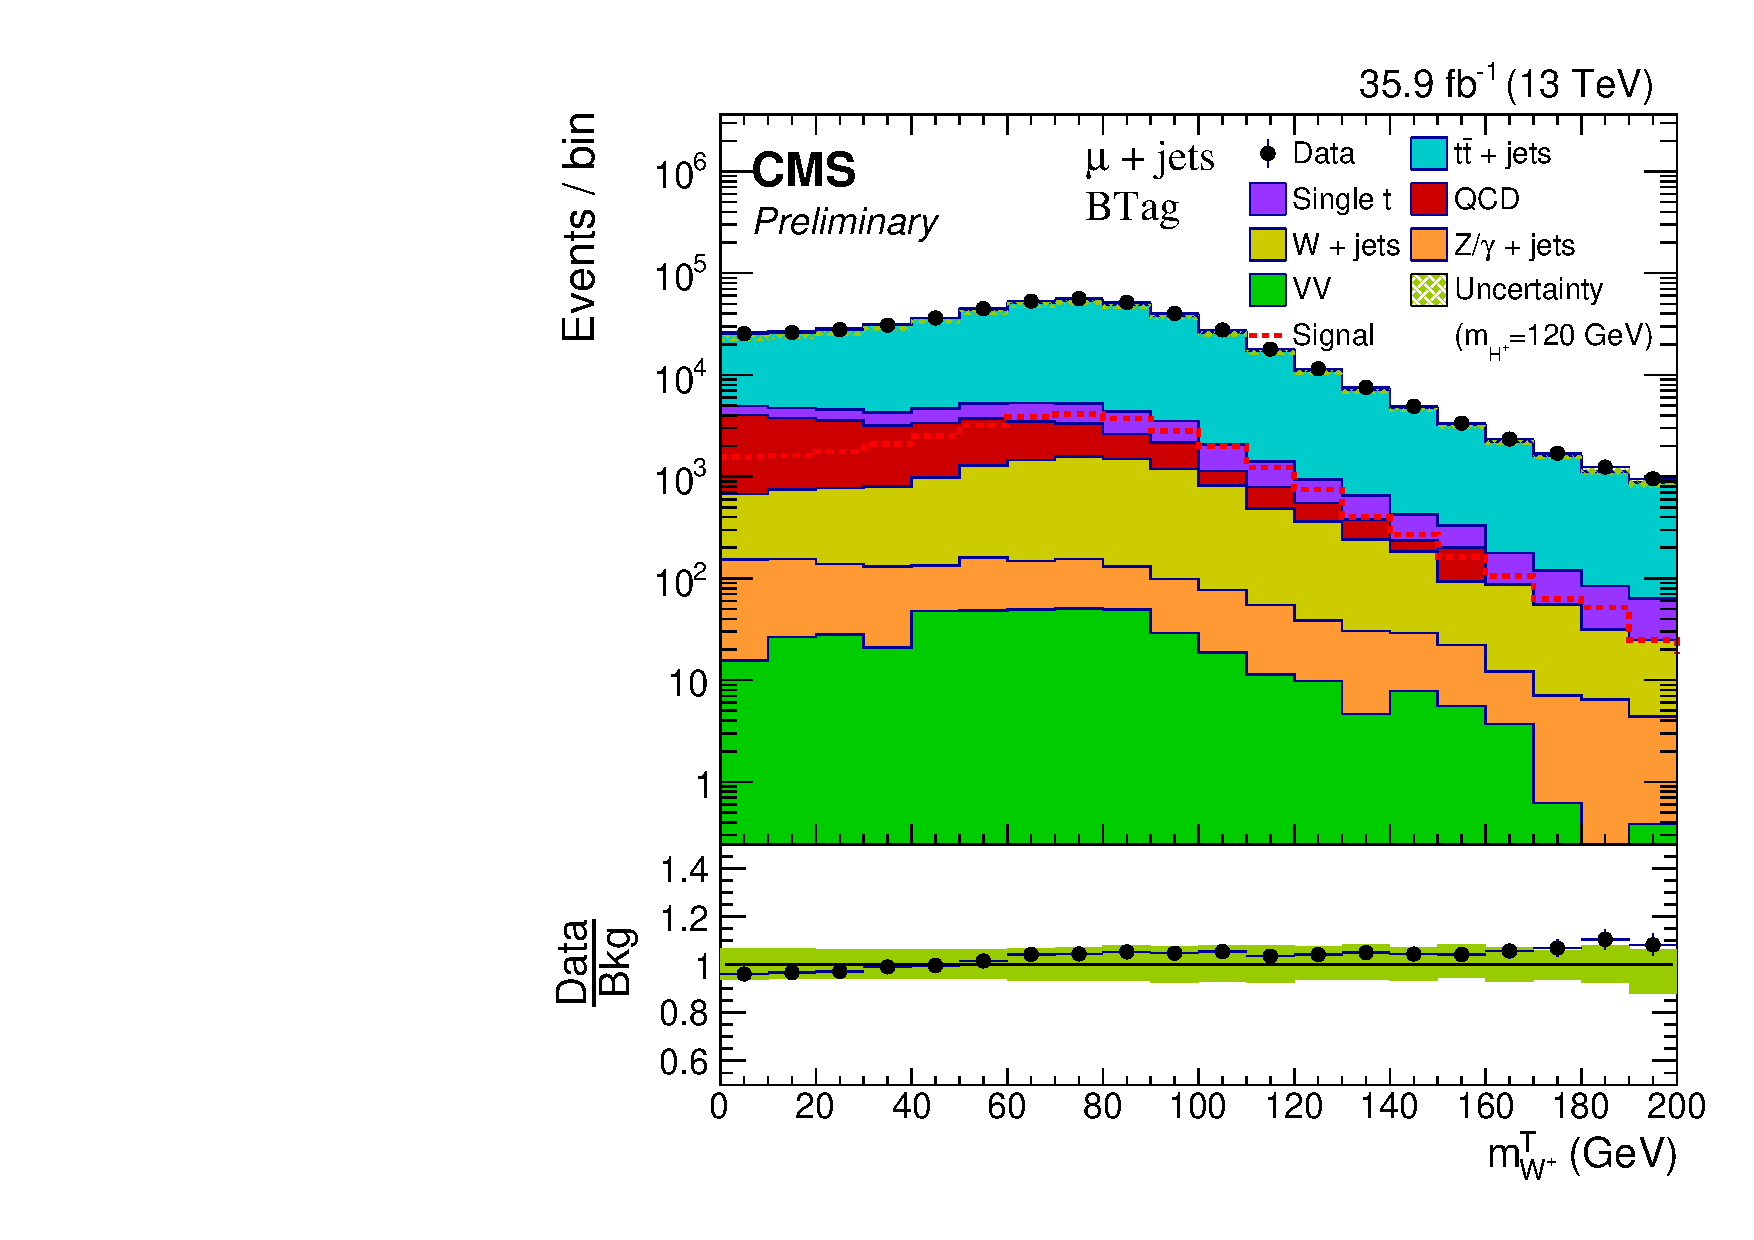
\includegraphics[width=0.45\linewidth]{Image/Muon/BTag/wmt_muBTag.pdf}}
    \subfigure[Transverse mass of \PW boson]{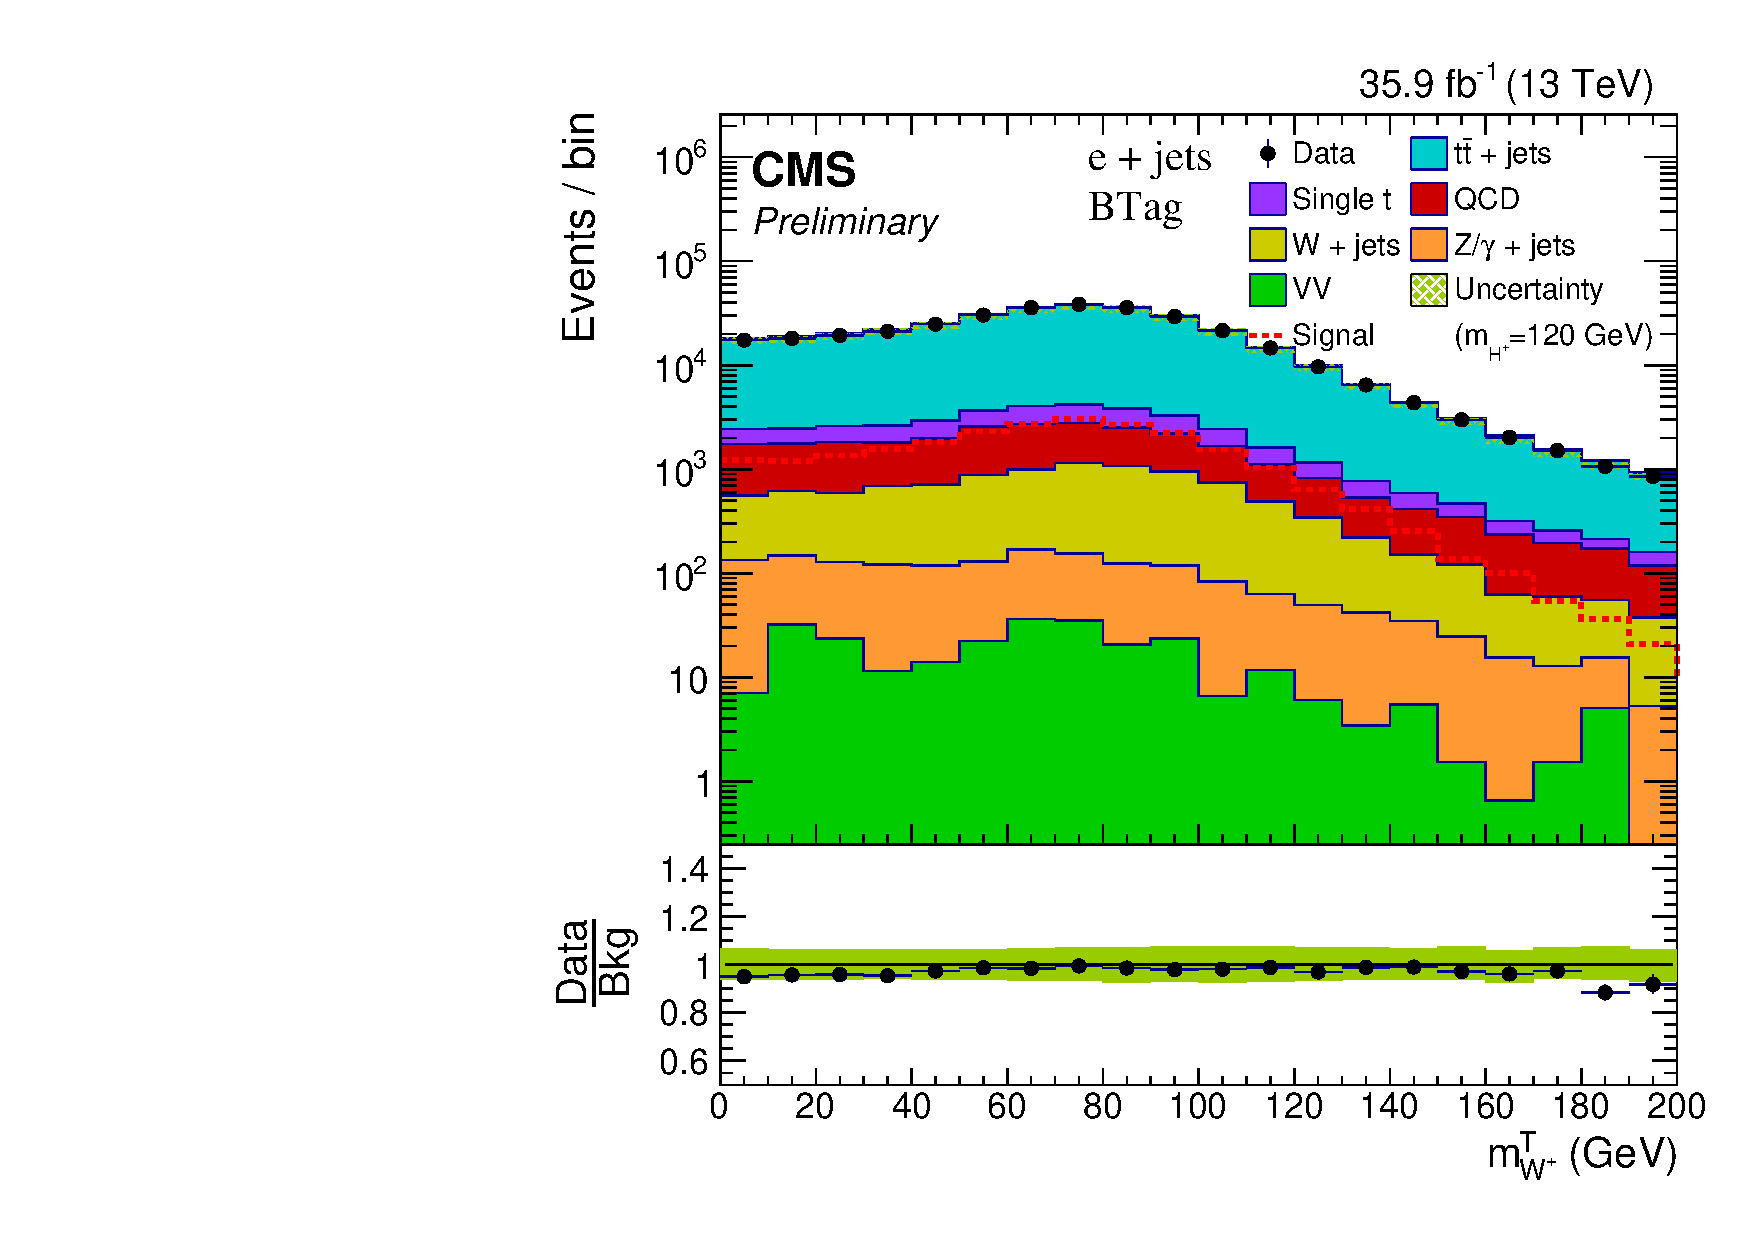
\includegraphics[width=0.45\linewidth]{Image/Electron/BTag/wmt_eleBTag.pdf}}
    \caption{Distribution of reconstructed $\MET$ and $m_{\PW^+}^{T}$ 
        (transverse mass of \PW boson decaying leptonically) after \PQb jet 
        selection as described in Section~\ref{s:secEvtSel}, for \mujets and 
    \ejets channel.}
    \label{fig:btagPlot3}
\end{figure}




